\pdfoutput=1
% ============================================================================
% GTOpt: open-source energy-system optimization, from minutes to decades
%
% Preprint (arXiv, eess.SY / math.OC); later target: IEEE Transactions on
% Power Systems.  Template: IEEEtran (journal mode).
%
% Overleaf-compatible: upload this entire directory as a project.
% To compile locally: latexmk -pdf main.tex
% ============================================================================

\documentclass[journal]{IEEEtran}

% ---- Encoding ----
\usepackage[utf8]{inputenc}
\usepackage[T1]{fontenc}

% ---- Math ----
\usepackage{amsmath,amssymb,amsfonts}

% ---- Graphics and tables ----
\usepackage{graphicx}
\usepackage{booktabs}
\usepackage{multirow}
\usepackage{tabularx}

% ---- Typography ----
\usepackage{textcomp}
\usepackage{xcolor}
\usepackage{siunitx}

% ---- Code listings ----
\usepackage{listings}
\lstset{
  basicstyle=\ttfamily\footnotesize,
  breaklines=true,
  frame=single,
  captionpos=b,
  numbers=left,
  numberstyle=\tiny\color{gray},
  xleftmargin=2em,
  framexleftmargin=1.5em,
}

% ---- Hyperlinks (load last among standard packages) ----
\usepackage[colorlinks=true,linkcolor=blue,citecolor=blue,urlcolor=blue,hypertexnames=false]{hyperref}
\usepackage{cite}

% ---- TikZ ----
\usepackage{tikz}
\usetikzlibrary{positioning,arrows.meta,shapes.geometric,fit,calc,patterns,decorations.pathreplacing}

% ---- Algorithms ----
\usepackage{algorithmic}
\usepackage{algorithm}

% ---- Custom commands ----
\newcommand{\gtopt}{GTOpt}
\newif\ifjournalversion
\journalversionfalse
\newcommand{\fesop}{FESOP}
\newcommand{\R}{\mathbb{R}}
\newcommand{\Z}{\mathbb{Z}}
\newcommand{\setS}{\mathcal{S}}
\newcommand{\setT}{\mathcal{T}}
\newcommand{\setB}{\mathcal{B}}
\newcommand{\setN}{\mathcal{N}}
\newcommand{\setG}{\mathcal{G}}
\newcommand{\setD}{\mathcal{D}}
\newcommand{\setL}{\mathcal{L}}
\newcommand{\setE}{\mathcal{E}}
\newcommand{\setJ}{\mathcal{J}}
\newcommand{\setR}{\mathcal{R}}
\newcommand{\setW}{\mathcal{W}}
\newcommand{\setH}{\mathcal{H}}
\newcommand{\setZ}{\mathcal{Z}}
\newcommand{\setFR}{\mathcal{F\!R}} % flow rights
\newcommand{\setVR}{\mathcal{V\!R}} % volume rights
\newcommand{\setHP}{\mathcal{H}_P}   % hydraulic pumps
\newcommand{\setLNG}{\mathcal{LNG}}  % LNG terminals
\newcommand{\setUC}{\mathcal{UC}}    % UC generators
\newcommand{\setIZ}{\mathcal{IZ}}    % inertia zones
\newcommand{\setIP}{\mathcal{IP}}    % inertia provisions

% ---- Graphics path ----
\graphicspath{{figures/}{diagrams/}}

% ============================================================================
\begin{document}

\title{%
  GTOpt: Open-Source Energy-System Optimization,\\
  Consistent from Minutes to Decades%
}

\author{%
  Marcelo~Matus~A.,~\IEEEmembership{Member,~IEEE,}
  Mar\'ia~del~Pilar~Buitrago~Villada,
  Erick~Sierra~Baeza,
  Carlos~Enrique~Garc\'ia~Bujanda,
  Marcos~Falcone~Salazar,
  and~Gonzalo~Bustos~Turu%
  \thanks{Preprint, November 2026.  Source code, data and documentation:
    \url{https://github.com/gtopt-community/gtopt}.}%
  \thanks{M.~Matus~A. is with Black Bear Engineering SpA, Santiago,
    Chile (\url{https://www.blackbeareng.cl}), and is a Fellow of
    Centro Enlace, Santiago, Chile (\url{https://centroenlace.org/})
    (e-mail: marcelo.matus@blackbear.cl).}%
  \thanks{M.~P.~Buitrago~Villada is with the Department of Electrical
    Energy and Automation, Universidad Nacional de Colombia,
    Medell\'in, Colombia.}%
  \thanks{E.~Sierra~Baeza is with Black Bear Engineering SpA, Santiago,
    Chile, and CENIA.}%
  \thanks{C.~E.~Garc\'ia~Bujanda is with Black Bear Engineering SpA,
    Santiago, Chile.}%
  \thanks{M.~Falcone~Salazar is with the School of Engineering,
    Universidad Adolfo Ib\'a\~nez, Santiago, Chile, and formerly with
    Colb\'un~S.A., Santiago, Chile.}%
  \thanks{G.~Bustos~Turu is with the Department of Chemical Engineering,
    Imperial College London, London, UK, and the Centre for Energy,
    Universidad de Chile, Santiago, Chile.}%
  % \thanks{Digital Object Identifier: 10.1109/TPWRS.20XX.XXXXXXX}%
}

% --- Create title and author block ---
\markboth{Preprint}%
  {Matus~A. \MakeLowercase{\textit{et al.}}: \gtopt{} for GTEP}

\maketitle

% ========== Abstract ==========
\begin{abstract}
Planning and operating energy systems with high shares of variable
renewables, storage and hydro requires models that remain consistent
from daily dispatch to multi-decade expansion.  This paper presents
GTOpt, an open-source optimizer written in C++26 for the expansion
planning of generation, transmission, storage and demand, hydrothermal
scheduling, and unit commitment and dispatch.  The same formulation is
used at every time scale, from 15-minute blocks to 30-year horizons.  It
covers DC power flow with Kirchhoff constraints and line losses, hydro
cascades with water rights, batteries, unit commitment, reserves and
inertia, multi-carrier chains (fuels, LNG, hydrogen, ammonia, heat)
and multi-pollutant emission zones with caps and allowance
banking.  The time scales are coupled through optimality cuts, which
carry water values and storage opportunity costs, and through
feasibility cuts, which enforce reservoir and water-right limits.  Three
methods are provided: a monolithic LP/MIP; stochastic dual
dynamic programming (SDDP) with backward-pass apertures, multi-cut and
elastic-filter feasibility cuts; and a multi-level cascade that refines
a coarse model into a detailed one while inheriting its cuts.  Operating
rules such as the Chilean irrigation agreements are added without code
through PAMPL, an AMPL-like constraint language, and LP/MIP solvers are
loaded at run time as plugins.  GTOpt is validated against IEEE
benchmark networks, pandapower and published SDDP benchmarks.  It is
also compared with the official daily schedule of the Chilean national
system on 14 days, using the system operator's PLEXOS inputs and
results.  The comparison shows that the line-loss model drives most of
the differences: a piecewise-linear loss model with free losses
inflates them to 2.5 times their physical value, whereas a tangent
outer approximation with a small loss price stays within 5\%.
\end{abstract}

% ========== Keywords ==========
\begin{IEEEkeywords}
Energy system optimization, generation and transmission expansion
planning, hydrothermal scheduling, stochastic dual dynamic programming,
multi-scale consistency, DC optimal power flow, line losses, energy
storage, water values, irrigation agreements, emissions, open-source
software.
\end{IEEEkeywords}

% ========== Sections ==========
% ============================================================================
% Section I: Introduction
% ============================================================================

\section{Introduction}
\label{sec:introduction}

The transition toward low-carbon energy systems requires planning tools
that co-optimize generation, transmission and storage investments while
capturing the operational detail of variable renewables, storage and
hydro cascades~\cite{lumbreras2016progressive}.  Generation and
Transmission Expansion Planning (GTEP) determines the minimum-cost
combination of investments (CAPEX) and operating decisions (OPEX) over
long horizons under
uncertainty~\cite{hemmati2013comprehensive, mahdavi2019tep_survey}.
In hydro-dominated systems the same questions extend to the medium term
(months to years), where reservoir management under inflow uncertainty
is solved with stochastic dual dynamic programming
(SDDP)~\cite{pereira1991sddp}, and to daily operation, where unit
commitment and network constraints set the dispatch and the marginal
prices.

In practice these three horizons are usually served by different
models, with different data formats, element definitions and
simplifications.  A long-term expansion model, a medium-term
hydrothermal model and a short-term scheduling model can therefore
disagree on the value of water, the opportunity cost of storage or the
feasibility of operating rules, and the policy handed from one horizon
to the next is only approximately consistent.  The commercial tools used
by system operators and utilities (e.g.\ PLEXOS, PSR SDDP, and in Chile
the PLP model maintained by the system operator) are closed or tied to
specific data formats, which limits the auditability of their results.
Open-source tools such as PyPSA~\cite{brown2018pypsa},
GenX~\cite{jenkins2017genx}, IDAES-GTEP~\cite{idaes_gtep2024} and
SDDP.jl~\cite{dowson2020sddp_jl} have broadened access to planning and
stochastic optimization.  None of them, however, combines in
one model a detailed hydro and water-rights representation, a network
with losses, SDDP and capacity expansion.

This paper presents GTOpt, an open-source optimizer for planning and
operating energy systems, written in C++26.  GTOpt descends from the
FESOP (Fabulous Energy System Optimizer)
framework~\cite{buitrago2022fesop}, which extended long-term
hydrothermal scheduling~\cite{pereira2016hydrothermal} with capacity
expansion, variable renewables and modern flexibility mechanisms.  Its
central design decision is to use \emph{one} formulation of the energy
system---electricity, water, fuels and LNG, hydrogen, ammonia and
heat---at every time scale, and to change only the time structure and
the solution method between scales.

The main contributions of this work are:

\begin{enumerate}
  \item A complete LP/MIP formulation of the energy system
    (Section~\ref{sec:formulation}).  It includes:
    \begin{itemize}
      \item DC optimal power flow with Kirchhoff constraints,
        transmission switching, zero-impedance ties, dynamic line
        rating through critical spans, and several line-loss models
        with a guard against loss arbitrage under negative prices;
      \item batteries with charge and discharge modes, and hydro
        cascades with reservoirs, turbines, pumps, seepage and
        head-dependent efficiency;
      \item a generic water-rights layer for irrigation agreements;
      \item typical periods and point-sampled stages on Chebyshev
        nodes, with storage balances consistent with the quadrature of
        energy and cost;
      \item unit commitment (three-binary energy-block and power-based
        formulations on chronological stages, a per-block formulation
        on load-duration stages) with
        piecewise heat rates and pricing modes, dynamic reserve
        requirements, battery reserve deliverability and synchronous
        inertia;
      \item LNG terminals and hydrogen, ammonia and heat chains;
      \item a natural-gas network with Weymouth pipes in squared
        pressure, elevation, compressor fuel, line pack, and
        gas-fired units limited by their fuel-gas pressure, with
        nodal gas prices (Section~\ref{sec:gas});
      \item multi-pollutant emission zones with caps, banking and
        carbon capture;
      \item multi-stage capacity expansion of generation, transmission,
        storage and demand.
    \end{itemize}

  \item A multi-scale design in which the same element definitions are
    used from 15-minute operation to 30-year planning, with the scales
    coupled through SDDP optimality and feasibility cuts
    (Section~\ref{sec:multiscale}).

  \item Three solution methods---monolithic LP/MIP; SDDP with
    apertures, multi-cut and elastic-filter feasibility cuts; and a
    multi-level cascade---plus an investment master over SDDP operation
    (Section~\ref{sec:methods}).

  \item An open software architecture (Section~\ref{sec:architecture}):
    \begin{itemize}
      \item JSON and Apache Parquet data, and PAMPL user constraints;
      \item run-time solver plugins and solver-neutral warm starts;
      \item exportable LP files with structural fingerprints;
      \item converters from PLP, PLEXOS, PSR SDDP, PSS/E, pandapower
        and open test-system formats;
      \item command-line, terminal-dashboard, browser and web-service
        interfaces.
    \end{itemize}

  \item Validation on IEEE benchmark networks, pandapower, published
    SDDP, unit-commitment, pricing and reserve benchmarks, and open gas
    and gas--electric test systems (Section~\ref{sec:validation}), and
    a comparison of
    GTOpt with the official daily schedule of the Chilean national
    system on 14 days, computed by the system operator with PLEXOS
    (Section~\ref{sec:cases}).
\end{enumerate}

The remainder of this paper is organized as follows.
Section~\ref{sec:literature} reviews the state of the art.
Section~\ref{sec:formulation} presents the formulation, and
Section~\ref{sec:gas} its natural-gas network.
Section~\ref{sec:methods} describes the solution methods and the
multi-scale coupling.  Section~\ref{sec:architecture} details the
software architecture.  Section~\ref{sec:validation} presents the
validation on benchmarks, and Section~\ref{sec:cases} the comparison
with the Chilean daily schedule.  Section~\ref{sec:conclusions}
concludes and outlines future work.

% ============================================================================
% Section II: Literature Review and State of the Art
% ============================================================================

\section{Literature Review}
\label{sec:literature}

\subsection{Generation and Transmission Expansion Planning}

GTEP is a classical problem in power systems that has been studied
extensively since the 1970s.  Romero et al.~\cite{romero2002test} provided
canonical test systems and mathematical models---including transportation,
hybrid, DC power flow, and disjunctive formulations---that remain standard
benchmarks.  Hemmati et al.~\cite{hemmati2013comprehensive} presented a
comprehensive review covering generation expansion planning (GEP),
transmission expansion planning (TEP), and their integration.  More
recently, Mahdavi et al.~\cite{mahdavi2019tep_survey} classified TEP
literature into categories by mathematical model, solution method, and
uncertainty handling, identifying a trend toward stochastic,
multi-objective, and market-based formulations.

Lumbreras and Ramos~\cite{lumbreras2016progressive} surveyed modern
challenges in TEP including renewable integration, energy storage, and
the need for multi-stage stochastic models.  These challenges motivate
the development of tools that can handle joint generation, transmission,
and storage expansion under operational uncertainty.

\subsection{DC Optimal Power Flow}

The DC power flow approximation linearizes the AC power flow equations
by assuming lossless lines, flat voltage profiles, and small angle
differences~\cite{stott2009dc_opf}.  Despite its simplifications, DC OPF
is the standard formulation for TEP because it yields a linear program
amenable to efficient solution~\cite{frank2016or_opf}.  Molzahn and
Hiskens~\cite{molzahn2019opf_survey} provided a comprehensive survey of
relaxations and approximations, confirming that DC OPF remains the
workhorse for expansion planning despite advances in convex relaxations
of AC OPF.

\gtopt{} adopts the $B$-$\theta$ formulation (susceptance-angle) for
DC OPF, as recommended by Stott et al.~\cite{stott2009dc_opf}, with
extensions for resistive losses via piecewise-linear approximations and
phase-shifting transformers.

\subsection{Stochastic Dual Dynamic Programming}

The Stochastic Dual Dynamic Programming (SDDP) algorithm, introduced by
Pereira and Pinto~\cite{pereira1991sddp}, is the standard method for
solving large-scale multi-stage stochastic programs in hydrothermal
scheduling.  The algorithm constructs piecewise-linear approximations of
the expected cost-to-go function through iterative forward and backward
passes.

Shapiro~\cite{shapiro2011sddp_analysis} provided theoretical convergence
analysis of SDDP, and Philpott and de~Matos~\cite{philpott2013sddp_convergence}
extended the algorithm with risk-averse sampling.  Recent advances include
batch learning SDDP~\cite{leclercq2023batch_sddp}, which frames the
algorithm as Q-learning for improved convergence, and extensions to
stochastic OPF under uncertainty~\cite{fletcher2024sddp_opf}.

In the Julia ecosystem, Dowson and Kapelevich~\cite{dowson2020sddp_jl}
developed SDDP.jl, a modular SDDP implementation, together with a set
of reference problems used here for validation
(Section~\ref{sec:validation}).  \gtopt{} provides a C++ SDDP
implementation with backward-pass apertures, multi-cut and Markov-chain
variants, elastic-filter feasibility cuts, and boundary cuts that couple
studies of different horizons (Section~\ref{sec:multiscale}).

\subsection{Energy Storage in Expansion Planning}

The integration of battery energy storage systems (BESS) into expansion
planning has received significant attention.  Go et al.~\cite{Go2016ess_expansion}
assessed the economic value of co-optimized grid-scale storage investments.
Frazier et al.~\cite{frazier2023bess_milp} presented an integrated MILP
for generation, transmission, and storage expansion with Benders
decomposition.

Sandia National Laboratories released QuESt Planning~\cite{sandia2024quest},
an open-source capacity expansion tool focused on storage, while
IDAES-GTEP~\cite{idaes_gtep2024} provides a modular Pyomo-based framework
for GTEP.  \gtopt{} supports BESS with detailed charge/discharge efficiency
modeling, state-of-charge tracking across stages, and co-located
generation-storage coupling via its converter mechanism.

\subsection{Integrated Gas and Electricity Networks}
\label{sec:lit_gas}

Steady-state gas transmission is governed by the Weymouth equation,
which is linear in the squared pressure and quadratic in the
flow~\cite{menon2005gas}.  De~Wolf and Smeers~\cite{dewolf2000gas}
solved the resulting gas transmission problem with an extension of the
simplex algorithm, and Tomasgard et al.~\cite{tomasgard2007gas}
approximated the Weymouth cone by tangent planes inside an LP of the
gas value chain.  R\'ios-Mercado and
Borraz-S\'anchez~\cite{riosmercado2015review} reviewed the optimization
problems of gas transportation, and Borraz-S\'anchez et
al.~\cite{borraz2016relaxations} proposed convex relaxations for
expansion planning.  On the power side, Liu et al.~\cite{liu2009scuc_gas}
added gas transmission constraints to security-constrained unit
commitment, and Correa-Posada and
S\'anchez-Mart\'in~\cite{correaposada2015gas} integrated both networks
in short-term operation.  Ordoudis et al.~\cite{ordoudis2019gas} and
Ratha et al.~\cite{ratha2020affine} cleared coupled electricity and gas
markets with tangent-plane Weymouth constraints and line pack, Hu and
Ryan~\cite{hu2019stochastic} compared stochastic and deterministic
scheduling of a coupled system, and Bent et al.~\cite{bent2018joint}
planned joint transmission expansion with market feedbacks.

Saldarriaga~\cite{saldarriaga2013msc, saldarriaga2013holistic,
saldarriaga2018phd, saldarriaga2019stochastic} developed integrated
planning models for gas and electricity, from distribution networks to
multi-stage stochastic transmission planning; his doctoral thesis
derives the compressor-fuel model adopted in Section~\ref{sec:gas}.
Later work of the same group addressed seasonal storage in integrated
systems~\cite{martinez2022storage} and the LNG supply
chain~\cite{ibarra2019gnl, restrepo2021gnl}.  Open tools and data
support this line of research: GasModels.jl~\cite{gasmodels} and
GasPowerModels.jl~\cite{gaspowermodels} implement exact and relaxed gas
formulations in Julia, and GasLib~\cite{schmidt2017gaslib,
pfetsch2015nominations} provides gas network instances.

Most of these models are nonlinear or mixed-integer, or they treat the
gas system as a separate market.  \gtopt{} instead keeps the gas
network as a pure LP inside the same multi-stage hydrothermal model:
exact tangent envelopes on radial networks, a sequential LP for meshed
ones, and compressor fuel as Taylor planes in the squared pressure.
The gas and power duals are therefore consistent, and the network can
be solved by SDDP together with reservoirs and storage.

\subsection{Open-Source Power System Tools}

Table~\ref{tab:tool_comparison} compares \gtopt{} with the leading
open-source GTEP tools.  PyPSA~\cite{brown2018pypsa} is the most widely
adopted, offering multi-sector coupling and a large community, and
targets linear expansion and dispatch rather than stochastic
hydrothermal scheduling.
GenX~\cite{jenkins2017genx} provides a flexible Julia/JuMP framework but
lacks native DC OPF and hydro cascade modeling.  pandapower~\cite{thurner2018pandapower}
excels at power flow analysis but does not support expansion planning.

\begin{table*}[t]
  \centering
  \caption{Comparison of Open-Source GTEP and Power System Tools}
  \label{tab:tool_comparison}
  \begin{tabular}{@{}lcccccc@{}}
    \toprule
    \textbf{Feature} & \textbf{GTOpt} & \textbf{PyPSA} & \textbf{GenX}
      & \textbf{IDAES-GTEP} & \textbf{QuESt} & \textbf{PLP} \\
    \midrule
    Language          & C++26  & Python  & Julia   & Python  & Python  & Fortran \\
    License           & AGPL-3\textsuperscript{a} & MIT & GPL-2 & BSD-3 & BSD-3 & --\textsuperscript{b} \\
    DC OPF (Kirchhoff)& \checkmark & \checkmark & Transport & \checkmark & -- & \checkmark \\
    Hydro cascades    & \checkmark & Partial & -- & -- & -- & \checkmark \\
    Battery storage   & \checkmark & \checkmark & \checkmark & Partial & \checkmark & Partial \\
    SDDP solver       & \checkmark & -- & -- & -- & -- & \checkmark \\
    Capacity expansion& \checkmark & \checkmark & \checkmark & \checkmark & \checkmark & -- \\
    Multi-scenario    & \checkmark & Partial & Partial & -- & -- & \checkmark \\
    Multi-sector      & \checkmark & \checkmark & Partial & -- & -- & -- \\
    Line losses       & \checkmark & \checkmark & \checkmark & -- & -- & \checkmark \\
    Water rights      & \checkmark & -- & -- & -- & -- & \checkmark \\
    Unit commitment   & \checkmark & \checkmark & \checkmark & \checkmark & -- & -- \\
    Emission caps     & \checkmark & \checkmark & \checkmark & -- & -- & -- \\
    Gas network (pressure) & \checkmark & Transport & -- & -- & -- & -- \\
    Cut-coupled scales& \checkmark & -- & -- & -- & -- & Partial \\
    Parquet I/O       & \checkmark & -- & -- & -- & -- & -- \\
    Web GUI           & \checkmark & -- & -- & -- & \checkmark & -- \\
    \bottomrule
  \end{tabular}
  \\[3pt]
  {\footnotesize \textsuperscript{a}AGPL-3.0-or-later with a solver-plugin
   exception, or commercial.
   \textsuperscript{b}Maintained by the Chilean system operator (CEN).}
\end{table*}

\gtopt{} distinguishes itself through:
\begin{enumerate}
  \item one formulation used from daily operation to multi-decade
    planning, with the time scales coupled by SDDP cuts;
  \item complete hydro cascade modeling with reservoirs, waterways,
    turbines, pumps and seepage;
  \item a generic water-rights layer for irrigation agreements with
    volume-dependent dynamic bounds;
  \item three solution methods, including SDDP and cascade
    decomposition;
  \item an auditable model: a published formulation, exportable LP
    files and structural fingerprints;
  \item native Apache Parquet I/O and converters from the commercial
    models used in the region.
\end{enumerate}

% ============================================================================
% Section III: Mathematical Formulation
% ============================================================================

\section{Mathematical Formulation}
\label{sec:formulation}

\subsection{Sets and Indices}

The GTEP problem is defined over the following sets:

\begin{itemize}
  \item $\setS$: scenarios, indexed by $s$, with probability $\pi_s$
  \item $\setT$: stages (planning periods), indexed by $t$
  \item $\setB_t$: blocks (operating periods) in stage $t$, indexed by $b$,
        with duration $\Delta_b$ [h]
  \item $\setN$: buses (electrical nodes), indexed by $n$
  \item $\setG$: generators, indexed by $g$, with bus $n_g$
  \item $\setD$: demands, indexed by $d$, with bus $n_d$
  \item $\setL$: transmission lines, indexed by $\ell$, connecting buses
        $a_\ell$ and $b_\ell$
  \item $\setE$: batteries (energy storage), indexed by $e$
  \item $\mathcal{V}$: converters (battery$\leftrightarrow$grid), indexed by $v$
  \item $\setJ$: hydraulic junctions, indexed by $j$
  \item $\setR$: reservoirs, indexed by $r$, with junction $j_r$
  \item $\setW$: waterways, indexed by $w$
  \item $\setH$: turbines, indexed by $h$
  \item $\setZ$: reserve zones, indexed by $z$
  \item $\mathcal{P}$: reserve provisions, indexed by $p$
  \item $\setFR$: flow rights (flow-based water rights), indexed by $i$
  \item $\setVR$: volume rights (volume-based water rights), indexed by $o$
  \item $\setHP$: hydraulic pumps, indexed by $h$
  \item $\setLNG$: LNG storage terminals, indexed by $\tau$
  \item $\setUC$: generators with unit commitment, indexed by $g$
  \item $\setIZ$: inertia zones, indexed by $z$
  \item $\setIP$: inertia provisions, indexed by $p$
\end{itemize}

\begin{figure}[t]
  \centering
  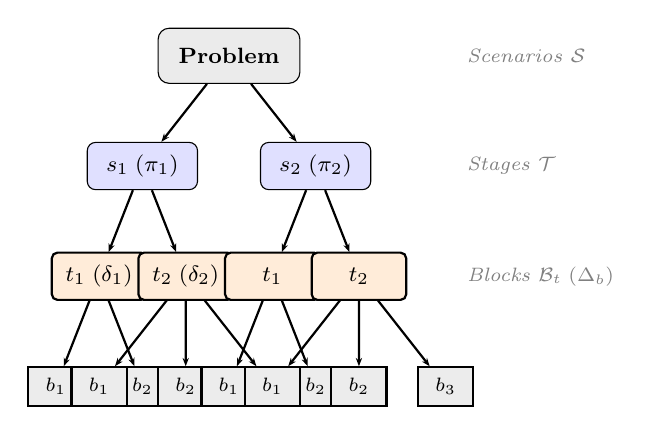
\begin{tikzpicture}[
    level 1/.style={sibling distance=22mm, level distance=14mm},
    level 2/.style={sibling distance=11mm, level distance=14mm},
    scen/.style={draw, rounded corners=3pt, fill=blue!12,
      font=\footnotesize, minimum width=14mm, minimum height=6mm},
    stg/.style={draw, rounded corners=2pt, fill=orange!15,
      font=\footnotesize, minimum width=12mm, minimum height=6mm},
    blk/.style={draw, fill=gray!15,
      font=\scriptsize, minimum width=7mm, minimum height=5mm},
    edge from parent/.style={draw, -{Stealth[length=3pt]}, thick},
    root/.style={draw, rounded corners=4pt, fill=black!8,
      font=\footnotesize\bfseries, minimum width=18mm,
      minimum height=7mm},
  ]
    \node[root] {Problem}
      child { node[scen] {$s_1\;(\pi_1)$}
        child { node[stg] {$t_1\;(\delta_1)$}
          child { node[blk] {$b_1$} }
          child { node[blk] {$b_2$} }
        }
        child { node[stg] {$t_2\;(\delta_2)$}
          child { node[blk] {$b_1$} }
          child { node[blk] {$b_2$} }
          child { node[blk] {$b_3$} }
        }
      }
      child { node[scen] {$s_2\;(\pi_2)$}
        child { node[stg] {$t_1$}
          child { node[blk] {$b_1$} }
          child { node[blk] {$b_2$} }
        }
        child { node[stg] {$t_2$}
          child { node[blk] {$b_1$} }
          child { node[blk] {$b_2$} }
          child { node[blk] {$b_3$} }
        }
      };
    % Level labels on the right
    \node[anchor=west, font=\scriptsize\itshape, text=black!50]
      at (2.9,0) {Scenarios $\setS$};
    \node[anchor=west, font=\scriptsize\itshape, text=black!50]
      at (2.9,-1.4) {Stages $\setT$};
    \node[anchor=west, font=\scriptsize\itshape, text=black!50]
      at (2.9,-2.8) {Blocks $\setB_t\;(\Delta_b)$};
  \end{tikzpicture}
  \caption{Three-level time hierarchy.  The problem decomposes into
    scenarios~$s$ (probability~$\pi_s$), stages~$t$ (discount
    factor~$\delta_t$), and blocks~$b$ (duration~$\Delta_b$).}
  \label{fig:time_hierarchy}
\end{figure}

\subsection{Decision Variables}

\noindent\textbf{Operational variables} (per scenario $s$, stage $t$, block $b$):
\begin{align}
  p_{g,s,t,b}  &\in [\underline{p}_g, \overline{p}_g]
    & \text{generator output [MW]} \label{eq:pgen} \\
  \ell_{d,s,t,b} &\in [0, \overline{\ell}_d]
    & \text{served demand [MW]} \label{eq:load} \\
  q_{d,s,t,b}  &\geq 0
    & \text{unserved demand [MW]} \label{eq:fail} \\
  f_{\ell,s,t,b} &\in [-\overline{F}^{ba}_\ell, \overline{F}^{ab}_\ell]
    & \text{line flow [MW]} \label{eq:flow} \\
  \theta_{n,s,t,b} &\in \R
    & \text{voltage angle [rad]} \label{eq:theta}
\end{align}

\noindent\textbf{Storage state variables}:
\begin{align}
  e_{e,s,t,b}  &\in [\underline{e}_e, \overline{e}_e]
    & \text{battery SoC [MWh]} \label{eq:soc} \\
  v_{r,s,t,b}  &\in [\underline{v}_r, \overline{v}_r]
    & \text{reservoir volume [hm\textsuperscript{3}]} \label{eq:vol} \\
  v_{\tau,s,t,b}^{\text{lng}}
               &\in [\underline{V}_\tau, \overline{V}_\tau]
    & \text{LNG tank volume [m\textsuperscript{3}]} \label{eq:lng_vol}
\end{align}

\noindent\textbf{Unit commitment variables} (per scenario $s$, stage $t$, period $p$):
\begin{align}
  u_{g,s,t,p} &\in \{0,1\} & \text{unit status (1 = online)} \\
  v_{g,s,t,p} &\in \{0,1\} & \text{startup event} \\
  w_{g,s,t,p} &\in \{0,1\} & \text{shutdown event}
\end{align}

\noindent\textbf{Investment variables} (per stage $t$):
\begin{equation}
  m_{g,t} \in [0, \overline{m}_g]
  \quad \text{expansion modules built} \label{eq:expmod}
\end{equation}

\subsection{Objective Function}

Minimize total expected discounted cost:
\begin{equation}
\label{eq:objective}
\min \sum_{s \in \setS} \pi_s \sum_{t \in \setT} \delta_t
\left[
  \sum_{b \in \setB_t} \Delta_b \cdot C^\text{op}_{s,t,b}
  + C^\text{inv}_t
\right]
\end{equation}
where $\delta_t = (1+r)^{-\tau_t/8760}$ is the discount factor with annual
rate $r$ and $\tau_t$ the cumulative hours to stage $t$.

The operational cost for each $(s,t,b)$ is:
\begin{multline}
\label{eq:opcost}
C^\text{op}_{s,t,b} = \sum_{g \in \setG} c_g \, p_{g,s,t,b}
  + \sum_{d \in \setD} c^f_d \, q_{d,s,t,b} \\
  + \sum_{\ell \in \setL} c_\ell
    (f^+_{\ell,s,t,b} + f^-_{\ell,s,t,b})
\end{multline}

The investment cost for stage $t$ is:
\begin{multline}
\label{eq:invcost}
C^\text{inv}_t = \sum_{g \in \setG} \omega^\text{cap}_{g,t} m_{g,t}
  + \sum_{d \in \setD} \omega^\text{cap}_{d,t} m_{d,t} \\
  + \sum_{\ell \in \setL} \omega^\text{cap}_{\ell,t} m_{\ell,t}
  + \sum_{e \in \setE} \omega^\text{cap}_{e,t} m_{e,t}
\end{multline}
where $\omega^\text{cap}_{(\cdot),t} = K_{(\cdot)} \delta_t T_t /
\sigma$ is the weighted investment cost coefficient,
$c_g$ is the variable generation cost [\$/MWh], $c^f_d$ is the
demand failure penalty [\$/MWh], $c_\ell$ is the transmission cost
[\$/MWh], $K_{(\cdot)}$ is the annualized investment cost
[\$/year] per module for each component, and $T_t$ is the stage
duration [h].  All objective coefficients are divided by a
scaling factor $\sigma$ (\texttt{scale\_objective}, default 1000) to
improve solver numerical conditioning.  Concretely, each operational LP
cost coefficient is weighted by $\omega_{s,t,b} = \pi_s \delta_t
\Delta_b / \sigma$, so the reported objective equals $z/\sigma$.

\subsection{Bus Power Balance}
\label{sec:balance}
\begin{multline}
\label{eq:balance}
\sum_{\substack{g \in \setG \\ n_g = n}} (1{-}\lambda_g) p_{g,s,t,b}
- \sum_{\substack{d \in \setD \\ n_d = n}}
  (1{+}\lambda_d)\,\ell_{d,s,t,b} \\
+ \sum_{\ell \in \setL} A_{n,\ell} \, f_{\ell,s,t,b} = 0
\end{multline}
where $\lambda_g, \lambda_d$ are injection and withdrawal loss factors,
respectively.  The line flow terms use directional contributions rather
than a simple incidence matrix: for each line~$\ell$ from bus~$a_\ell$
to~$b_\ell$, the sending bus sees $-f^+_\ell$ (or $+(1-\lambda_\ell)
f^-_\ell$ when losses are modeled) and the receiving bus sees
$+(1-\lambda_\ell)f^+_\ell$ (or $-f^-_\ell$), where $\lambda_\ell$
is the line loss factor.  When $\lambda_\ell=0$, a single bidirectional
variable suffices and the incidence reduces to $A_{n,\ell} \in
\{+1,-1,0\}$.  The dual of~\eqref{eq:balance} is the locational marginal
price (LMP) at bus~$n$.

\subsection{Demand Balance}

When demand curtailment is allowed, served and unserved demand sum to the
scheduled load:
\begin{equation}
\label{eq:demand_balance}
\ell_{d,s,t,b} + q_{d,s,t,b} = \overline{\ell}_{d,t,b}
\quad \forall\; d, s, t, b
\end{equation}
where $\overline{\ell}_{d,t,b}$ is the scheduled demand at block~$b$,
incorporating any demand profile scaling.  When curtailment is disabled,
the load is fixed: $\ell_{d,s,t,b} = \overline{\ell}_{d,t,b}$.

Instead of the single penalty $c^f_d$, a demand can carry a stepwise
value-of-lost-load curve of $K$ segments (\texttt{fail\_segments}): the
served load is split into $K$ tranches bounded by
$f_{d,k}\,\overline{\ell}_{d,t,b}$, and the curtailment of tranche~$k$
is priced at $c^f_{d,k}$.  With non-decreasing segment costs the LP
curtails the cheapest segment first, so the curve needs no extra rows,
ordering constraints or binaries.

\subsection{DC Power Flow (Kirchhoff Constraints)}

When \texttt{use\_kirchhoff} is enabled, for each line $\ell$ and
$(s,t,b)$:
\begin{equation}
\label{eq:kirchhoff}
f_{\ell,s,t,b} = \frac{V_\ell^2}{X_\ell}
  \left(\theta_{a_\ell,s,t,b} - \theta_{b_\ell,s,t,b}\right)
\end{equation}
where $X_\ell$ is the line reactance [$\Omega$] and $V_\ell$ is the
nominal voltage [kV].  The angle variables are enlarged by a factor
$\sigma_\theta$ (\texttt{scale\_theta}) for numerical conditioning:
$\theta^\text{LP} = \sigma_\theta \cdot \theta$.  When it is not set,
$\sigma_\theta = 1 / \bigl(3 \operatorname{median}_\ell (X_\ell /
V_\ell^2)\bigr)$.  An angle accumulates about $D$ line drops on the way
to the reference bus, and the factor $3 \approx \sqrt{D}$ balances the
angle coefficient of the Kirchhoff row against the size of
$\theta^\text{LP}$.  A value set by the user is kept as given.

A line with zero reactance, or with $|X_\ell/V_\ell^2|$ below a
threshold (default $10^{-6}$~p.u.), is a zero-impedance tie by default:
the flow term of~\eqref{eq:transformer} vanishes, the two bus angles are
forced equal (up to the phase shift), and the flow is free within the
line limits.  A line without a reactance is a DC link and has no
Kirchhoff row.

Line flow is bounded by transfer capacities:
\begin{equation}
-\overline{F}^{ba}_\ell \leq f_{\ell,s,t,b}
  \leq \overline{F}^{ab}_\ell
\end{equation}

\paragraph{Loop-flow formulation and switching.}
Besides the angle-based form~\eqref{eq:kirchhoff}, Kirchhoff's voltage
law can be written over a cycle basis of the network (one row per
independent loop, with no angle variables), which is smaller for
radial-heavy systems.  Lines can be declared switching candidates with a
binary state; the Kirchhoff row of a switchable line (or of every cycle
through it) is relaxed with a big-M disjunction, giving optimal
transmission switching as a MIP.

\paragraph{Transformer model.}
For tap-changing and phase-shifting transformers, the Kirchhoff
constraint generalizes to:
\begin{equation}
\label{eq:transformer}
-\theta_{a_\ell} + \theta_{b_\ell}
  + (\tau_\ell \chi_\ell)(f^+_\ell - f^-_\ell)
  = -\sigma_\theta \, \psi_{\ell}
\end{equation}
where $\tau_\ell$ is the off-nominal tap ratio (default~1),
$\chi_\ell = \sigma_\theta X_\ell / V_\ell^2$ is the scaled reactance,
and $\psi_\ell$ is the phase-shift angle [rad].
When $\tau_\ell = 1$ and $\psi_\ell = 0$,~\eqref{eq:transformer}
reduces to~\eqref{eq:kirchhoff}.

\subsection{Line Losses}
\label{sec:losses}

Losses are modeled with one of several formulations, selected per line
or system-wide.

\paragraph{Linear and piecewise models.}
The linear model splits the flow into forward and reverse components
$f^+_\ell, f^-_\ell \geq 0$; the receiving bus sees
$(1-\lambda_\ell)$ of the power sent.  The piecewise model approximates
the quadratic loss $R_\ell f^2 / V_\ell^2$ with $K$ equal segments per
direction, so the loss slope increases with the flow.

\paragraph{Loss arbitrage.}
Both models are exact only when the LP has no incentive to lose
energy.  When the sum of the duals of the two end buses is negative,
$\pi_{a_\ell} + \pi_{b_\ell} < 0$, which happens with curtailed
renewables, inflexible units or congestion with angular coupling, the
LP can fill expensive segments first or circulate flow in both
directions at once.  The losses then become a fictitious energy sink
that sets prices at zero instead of letting them become negative.
Section~\ref{sec:cases} shows the size of this effect on the Chilean
system.

\paragraph{Tangent outer approximation with a loss price.}
The \texttt{tangent\_signed\_flow} model uses a signed flow
$f_\ell$ and a loss variable $\lambda^{\mathrm{L}}_\ell$ bounded below
by $K$ tangents of the convex quadratic~\cite{coffrin2014lpac},
\begin{equation}
\label{eq:loss_tangent}
\lambda^{\mathrm{L}}_{\ell,s,t,b} \geq 2 c_\ell f^{(k)}_\ell
  f_{\ell,s,t,b} - c_\ell \bigl(f^{(k)}_\ell\bigr)^2,
  \quad k = 1,\dots,K,
\end{equation}
with $c_\ell = R_\ell/V_\ell^2$.  It is bounded above by a secant chord
on an auxiliary $v_\ell \geq |f_\ell|$, which closes the
bidirectional-flow channel.  A small loss price $\varepsilon_\ell$
[\$/MWh] on $\lambda^{\mathrm{L}}_\ell$, weighted by
$\omega_{s,t,b}$, removes the remaining incentive to inflate the losses
whenever $\varepsilon_\ell \geq \tfrac12 |\pi_{a_\ell}+\pi_{b_\ell}|$.
Its effect on legitimate operation is proportional to the losses, not to
the flow.  The same price is applied to the loss columns of the
piecewise and bidirectional models, where it also breaks the degeneracy
between one-way and two-way flow.  It defaults to 0.1~\$/MWh, can be
raised per line on the corridors where the arbitrage appears, and is
disabled with $\varepsilon_\ell = 0$.
For lines where the chord is too loose, an $L$-segment chord
with a type-2 special ordered set makes the upper bound tight at the
breakpoints, with a worst-case error of
$c_\ell \overline{F}_\ell^2/(4L^2)$.

\subsection{Battery Energy Storage}
\label{sec:battery}

State-of-charge balance for battery $e$ between consecutive blocks:
\begin{multline}
\label{eq:soc_balance}
e_{e,s,t,b} = e_{e,s,t,b-1}(1 - \mu_e^h \Delta_b) \\
  + p^\text{in}_{e,s,t,b} \cdot \eta^\text{in}_e \cdot \Delta_b
  - p^\text{out}_{e,s,t,b} \cdot \Delta_b / \eta^\text{out}_e
\end{multline}
where $\eta^\text{in}_e$ and $\eta^\text{out}_e$ are charge and discharge
efficiencies, $p^\text{in}, p^\text{out}$ are charge and discharge
power [MW], and $\mu_e^h = \mu_e / 8760$ is the hourly self-discharge
rate derived from the annual standing-loss rate~$\mu_e$
(\texttt{annual\_standing\_loss}, default 0.48~p.u./year, about 4\% per
month).
Initial SoC $e_{e,\cdot,\cdot,0} = e^\text{ini}_e$ is an
equality constraint in the first stage; the final SoC of stage~$t$
links to the initial SoC of stage~$t{+}1$.

\begin{figure}[t]
  \centering
  \resizebox{\columnwidth}{!}{%
  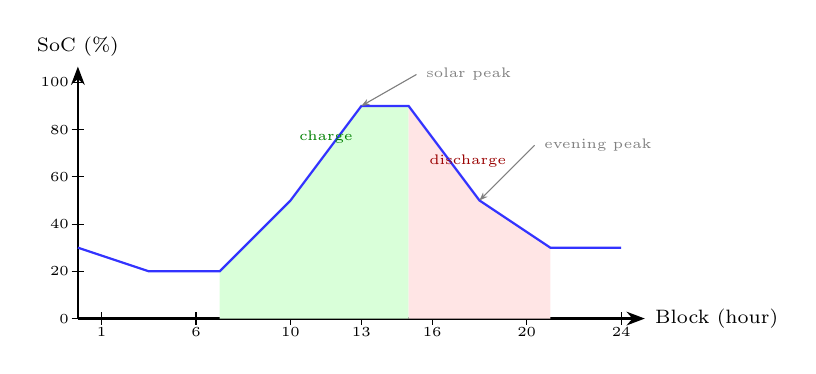
\begin{tikzpicture}[
    >=Stealth,
    axis/.style={->, thick},
    charge/.style={fill=green!15},
    discharge/.style={fill=red!10},
  ]
    % Axes
    \draw[axis] (0,0) -- (7.2,0)
      node[right, font=\scriptsize] {Block (hour)};
    \draw[axis] (0,0) -- (0,3.2)
      node[above, font=\scriptsize] {SoC (\%)};

    % Y-axis ticks
    \foreach \y/\lbl in {0/0, 0.6/20, 1.2/40, 1.8/60, 2.4/80, 3.0/100} {
      \draw (-0.08,\y) -- (0.08,\y)
        node[left=2pt, font=\tiny] {\lbl};
    }
    % X-axis ticks
    \foreach \x/\lbl in
      {0.3/1, 1.5/6, 2.7/10, 3.6/13, 4.5/16, 5.7/20, 6.9/24} {
      \draw (\x,-0.08) -- (\x,0.08)
        node[below=2pt, font=\tiny] {\lbl};
    }

    % SoC data points
    \coordinate (p0) at (0.0, 0.9);   % hour 0:  30%
    \coordinate (p1) at (0.9, 0.6);   % hour 3:  20%
    \coordinate (p2) at (1.8, 0.6);   % hour 6:  20%
    \coordinate (p3) at (2.7, 1.5);   % hour 10: 50%
    \coordinate (p4) at (3.6, 2.7);   % hour 13: 90%
    \coordinate (p5) at (4.2, 2.7);   % hour 15: 90%
    \coordinate (p6) at (5.1, 1.5);   % hour 18: 50%
    \coordinate (p7) at (6.0, 0.9);   % hour 21: 30%
    \coordinate (p8) at (6.9, 0.9);   % hour 24: 30%

    % Charge shading (hours 6--15)
    \fill[charge] (p2) -- (p3) -- (p4) -- (p5)
      -- (p5 |- 0,0) -- (p2 |- 0,0) -- cycle;

    % Discharge shading (hours 15--21)
    \fill[discharge] (p5) -- (p6) -- (p7)
      -- (p7 |- 0,0) -- (p5 |- 0,0) -- cycle;

    % SoC line
    \draw[thick, blue!80] (p0) -- (p1) -- (p2) -- (p3) -- (p4)
      -- (p5) -- (p6) -- (p7) -- (p8);

    % Labels
    \node[font=\tiny, green!50!black, above] at (3.15,2.1)
      {charge};
    \node[font=\tiny, red!60!black, above] at (4.95,1.8)
      {discharge};

    % Solar peak annotation
    \draw[{Stealth[length=3pt]}-, thin, gray]
      (3.6,2.7) -- (4.3,3.1)
      node[right, font=\tiny] {solar peak};

    % Evening peak annotation
    \draw[{Stealth[length=3pt]}-, thin, gray]
      (5.1,1.5) -- (5.8,2.2)
      node[right, font=\tiny] {evening peak};
  \end{tikzpicture}}%
  \caption{Battery SoC over 24~blocks: charge during solar hours (green),
    discharge during evening peak (red).}
  \label{fig:battery_soc}
\end{figure}

\subsection{Converter Constraints}

A converter~$v$ couples a battery~$e$ to the electrical network through
a generator~$g$ (discharge path) and a demand~$d$ (charge path) via a
power conversion rate~$\rho_v$:
\begin{align}
\label{eq:conv_discharge}
p_{g,s,t,b} &= \rho_v \cdot p^\text{out}_{e,s,t,b} \\
\label{eq:conv_charge}
\ell_{d,s,t,b} &= \rho_v \cdot p^\text{in}_{e,s,t,b}
\end{align}
When the converter has a capacity limit~$\overline{C}_v$, a joint bound
applies: $p_{g,s,t,b} + \ell_{d,s,t,b} \leq \bar{C}_{v,t}$.
Converter capacity is expandable using the same modular framework
as~\eqref{eq:capacity}.

\subsection{Hydro Cascade}
\label{sec:hydro}

For each junction $j$ with reservoir $r$, the water balance is:
\begin{multline}
\label{eq:hydro_balance}
v_{r,s,t,b} = v_{r,s,t,b-1} \\
  + \alpha_r \Delta_b \!\Bigl(
    \textstyle\sum_{w \in \text{in}(j)} q_{w}
    - \textstyle\sum_{w \in \text{out}(j)} q_{w}
    + F_j
  \Bigr)
\end{multline}
where $q_w$ is the waterway discharge [m$^3$/s], $F_j$ is the exogenous
inflow at junction $j$, and $\alpha_r = 0.0036$ converts flow rates to
volume increments: since 1~m$^3$/s flowing for 1~hour equals
3600~m$^3$ = 0.0036~hm$^3$, $\alpha_r = 3.6 \times 10^{-3}$
[hm$^3$/(m$^3$/s$\cdot$h)] (the default when \texttt{flow\_conversion\_rate}
is not set).  A junction can release surplus water through a drain
column bounded by a capacity and priced, like waterway flows and
spillways, per (m$^3$/s)$\cdot$h with the block weight
$\omega_{s,t,b}$.  These exit costs are optional.  When every exit of a
full reservoir carries a cost~$c$, its water value (the dual
of~\eqref{eq:hydro_balance}) is $-c/\alpha_r$: one more hm$^3$ must be
discharged at a cost, and SDDP carries such negative values through its
cuts.

Each turbine $h$ linking waterway $w$ to generator $g$ provides:
\begin{equation}
\label{eq:turbine}
p_{g,s,t,b} \leq \rho_h \cdot q_{w,s,t,b}
\end{equation}
where $\rho_h$ is the water-to-power conversion rate [MW$\cdot$s/m$^3$].

\paragraph{Volume-dependent turbine efficiency.}
In practice, the conversion rate depends on the hydraulic head, which
varies with reservoir volume.  When defined, $\rho_h$ is replaced by a
concave piecewise-linear function:
\begin{equation}
\label{eq:vol_efficiency}
\rho_h(v) = \min_{i=1}^{N}
  \bigl\{ c_i + m_i (v - v_i) \bigr\}
\end{equation}
where $(v_i, m_i, c_i)$ are volume breakpoints, slopes, and intercepts
of~$N$ segments.  In the SDDP method, the active segment is updated at
each forward-pass iteration using the current reservoir volume.

\paragraph{Filtration (seepage).}
Seepage from a waterway into a reservoir is modeled as a linear function
of the average volume:
\begin{equation}
\label{eq:filtration}
\varphi_{i,s,t,b} = a_i + b_i \cdot
  \frac{v_{r,s,t,b-1} + v_{r,s,t,b}}{2}
\end{equation}
where $a_i$ is a constant term and $b_i$ is the seepage rate per unit
volume.  As with turbine efficiency, this admits a piecewise-linear
extension selected by the last known volume.

\begin{figure}[t]
  \centering
  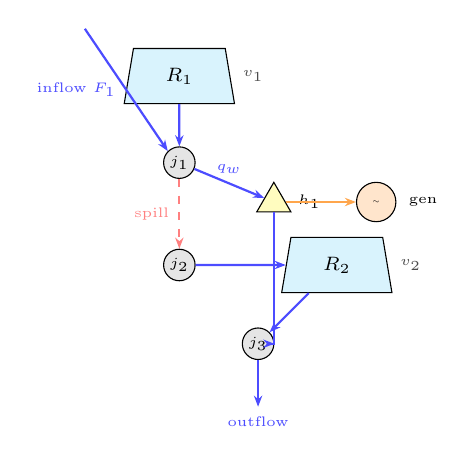
\begin{tikzpicture}[
    res/.style={trapezium, trapezium angle=75, draw, fill=cyan!15,
      minimum width=1.4cm, minimum height=0.7cm, font=\scriptsize,
      trapezium stretches body},
    junc/.style={circle, draw, fill=gray!20, minimum size=0.4cm,
      font=\tiny, inner sep=1pt},
    turb/.style={regular polygon, regular polygon sides=3, draw,
      fill=yellow!25, minimum size=0.5cm, font=\tiny, inner sep=0pt},
    gen/.style={circle, draw, fill=orange!20, minimum size=0.5cm,
      font=\tiny},
    flow/.style={-{Stealth[length=4pt]}, thick, blue!70},
    spill/.style={-{Stealth[length=4pt]}, thick, red!50, dashed},
  ]
    % Reservoir 1
    \node[res] (r1) at (0,2.2) {$R_1$};
    \node[font=\tiny\itshape, text=black!70, right=1pt of r1] {$v_1$};

    % Junction 1
    \node[junc] (j1) at (0,1.1) {$j_1$};

    % Inflow
    \draw[flow] (-1.2,2.8) -- (j1.north west)
      node[midway, left, font=\tiny] {inflow $F_1$};

    % R1 -> J1
    \draw[flow] (r1) -- (j1);

    % Turbine
    \node[turb] (t1) at (1.2,0.6) {};
    \node[font=\tiny, right=1pt of t1] {$h_1$};

    % Junction 2
    \node[junc] (j2) at (0,-0.2) {$j_2$};

    % J1 -> T1
    \draw[flow] (j1) -- (t1) node[midway, above, font=\tiny] {$q_w$};

    % T1 -> Generator
    \node[gen] (g1) at (2.5,0.6) {\raisebox{-0.5pt}{\scalebox{0.5}{$\sim$}}};
    \node[font=\tiny, right=1pt of g1] {gen};
    \draw[-{Stealth[length=4pt]}, thick, orange!70] (t1) -- (g1);

    % J1 -> J2 spillway
    \draw[spill] (j1) -- (j2) node[midway, left, font=\tiny] {spill};

    % Reservoir 2
    \node[res] (r2) at (2,-0.2) {$R_2$};
    \node[font=\tiny\itshape, text=black!70, right=1pt of r2] {$v_2$};

    % Junction 3
    \node[junc] (j3) at (1,-1.2) {$j_3$};

    % J2 -> R2 waterway
    \draw[flow] (j2) -- (r2);

    % T1 -> J3 (tailwater)
    \draw[flow] (t1) |- (j3);

    % R2 -> J3
    \draw[flow] (r2) -- (j3);

    % Outflow
    \draw[flow] (j3) -- (1,-2.0) node[below, font=\tiny] {outflow};
  \end{tikzpicture}
  \caption{Hydro cascade example: two reservoirs ($R_1$, $R_2$),
    three junctions ($j_1$--$j_3$), one turbine ($h_1$) driving a
    generator, with inflow, spillway, and waterway connections.}
  \label{fig:hydro_cascade}
\end{figure}

\subsection{Capacity Expansion}

Installed capacity evolves as:
\begin{equation}
\label{eq:capacity}
\bar{C}_{g,t} = \bar{C}_{g,t-1}(1-\xi_{g,t}) + M_g \cdot m_{g,t}
\end{equation}
where $\bar{C}_{g,0}$ is the initial installed capacity, $\xi_{g,t}$ is
the stage derating factor, $M_g$ is the capacity per expansion module
(\texttt{expcap}), and $m_{g,t}$ is the number of modules built.  The
generator output is bounded by the installed capacity:
\begin{equation}
p_{g,s,t,b} \leq \bar{C}_{g,t}
\end{equation}
Analogous expansion constraints apply to demands, lines, batteries, and
converters.

\subsection{Generator Profile Constraints}

When a generator has a capacity profile $\phi_g(s,t,b)$ (e.g., solar
irradiance or wind availability), the profile bounds the output.  The
profile is a per-unit factor of the capacity, and the available power is
capped by the generation range $\overline{p}_{g,t,b}$:
\begin{equation}
\label{eq:profile}
p_{g,s,t,b} \leq A_{g,s,t,b}
  = \min\bigl(\phi_g(s,t,b) \cdot \bar{C}_{g,t},\;
    \overline{p}_{g,t,b}\bigr)
\end{equation}
When the capacity is an expansion variable the row reads
$p_{g,s,t,b} - \min(\phi_g, 1)\,\bar{C}_{g,t} \leq 0$.  Curtailment
needs no variable of its own: the spilled renewable energy is computed
after the solve as $s_{g,s,t,b} = \max(0, A_{g,s,t,b} - p_{g,s,t,b})$,
and its marginal value is the dual of~\eqref{eq:profile}.  Only when
curtailment carries a cost $c_g^\text{spill}$ is the equality
$p_{g,s,t,b} + s_{g,s,t,b} = A_{g,s,t,b}$ with
$0 \leq s_{g,s,t,b} \leq A_{g,s,t,b}$ and cost
$c_g^\text{spill}\,\omega_{s,t,b}\,s_{g,s,t,b}$ used instead.

\subsection{Demand Minimum Energy}

An optional minimum energy constraint ensures that a demand~$d$ is
served a minimum total energy within each stage:
\begin{equation}
\label{eq:min_energy}
\sum_{b \in \setB_t} \ell^\text{man}_{d,s,t,b} \cdot \Delta_b
  \geq E_d^\text{min}
\end{equation}
where $\ell^\text{man}_{d,s,t,b}$ is the mandatory served load and
$E_d^\text{min}$ [MWh] is the stage energy requirement.

\subsection{Reserve Constraints}
\label{sec:reserve}

For each reserve zone $z$ and $(s,t,b)$:
\begin{equation}
\label{eq:reserve_up}
\sum_{p \in \mathcal{P}_z} \gamma_{p,t} \, r^\text{up}_{p,s,t,b}
  + q^\text{up}_{z,s,t,b}
  \geq R^\text{up}_{z,s,t,b}
\end{equation}
where $r^\text{up}_{p,s,t,b}$ is the up-reserve provision from
provision~$p$, $\gamma_{p,t}$ is the provision factor (typically~1),
$q^\text{up}_{z,s,t,b}$ is unserved reserve, and
$R^\text{up}_{z,s,t,b}$ is the zone requirement.  A symmetric constraint
exists for down-reserve.  Reserve provision is bounded by the generator's
headroom: $p_{g,s,t,b} + r^\text{up}_{p,s,t,b} \leq \bar{C}_{g,t}$.

\subsection{Hydro Pump}
\label{sec:pump}

A \texttt{Pump} element $h \in \setHP$ models a hydraulic pump
that consumes electrical power from a demand $d$ and raises water
through a waterway $w$ from a downstream junction to an upstream
junction---the reverse of a turbine.  The conversion constraint ties
the electrical load to the pumped flow:
\begin{equation}
\label{eq:pump}
\frac{\phi_{h,t}}{\eta_{h,t}} \, \varphi_{w,s,t,b} \leq \ell_{d,s,t,b}
\qquad \forall\, h \in \setHP,\; s,t,b
\end{equation}
where $\phi_{h,t}$ [MW/(m\textsuperscript{3}/s)] is the pump factor,
$\eta_{h,t} \in (0,1]$ is the stage efficiency, $\varphi_{w,s,t,b}$
[m\textsuperscript{3}/s] is the waterway flow, and
$\ell_{d,s,t,b}$ [MW] is the served electrical load.  An optional
capacity constraint bounds the flow:
$\varphi_{w,s,t,b} \leq \overline{Q}_{h,t}$.

The pump element only adds coupling rows to the LP; the waterway
retains its junction water balance contribution (Section~\ref{sec:hydro})
and the demand retains its bus power balance contribution
(Section~\ref{sec:balance}).  Reversible turbine-pump units (e.g.
pump-storage hydro) are modeled as a pair of elements: a
\texttt{Turbine} on the generation waterway and a \texttt{Pump} on the
pumping waterway.  Economic optimality (round-trip efficiency
$< 1.0$) prevents simultaneous generation and pumping without
explicit binary exclusivity constraints.

\subsection{LNG Terminal}
\label{sec:lng}

An \texttt{LngTerminal} element $\tau \in \setLNG$ models an
LNG storage tank whose inventory is coupled to gas-fired generators
through their heat rates.  The tank volume balance mirrors the battery
SoC equation (Section~\ref{sec:battery}) with delivery inflow and
boil-off:
\begin{multline}
\label{eq:lng_balance}
v_{\tau,s,t,b}^{\text{lng}}
  = v_{\tau,s,t,b-1}^{\text{lng}} \bigl(1 - \lambda_\tau^h \Delta_b\bigr)
  + \rho_\tau \Delta_b \, d_{\tau,s,t,b}^{\text{lng}} \\
  - \rho_\tau \Delta_b \, \text{vent}_{\tau,s,t,b}
  - \rho_\tau \Delta_b
      \sum_{g \in \mathcal{G}_\tau} \kappa_g^{hr} \, p_{g,s,t,b}
\end{multline}
where $v_{\tau,s,t,b}^{\text{lng}}$ [m\textsuperscript{3}] is the tank
volume, $\lambda_\tau^h = \lambda_\tau / 8760$ is the per-hour
boil-off rate, $\rho_\tau$ is a dimensionless unit-conversion factor
(default~1.0, used when delivery is in m\textsuperscript{3}/h and volume
in m\textsuperscript{3} so that $\rho_\tau \cdot \Delta_b \cdot d$ has
units m\textsuperscript{3}),
$d_{\tau,s,t,b}^{\text{lng}}$ is the delivery inflow, $\text{vent}$
is a vented-gas variable penalized at `spillway\_cost', and
$\kappa_g^{hr}$ [m\textsuperscript{3}/MWh] is the heat rate of each
linked generator $g \in \mathcal{G}_\tau$.

The last term is implemented by injecting a coefficient
$-\rho_\tau \kappa_g^{hr} \Delta_b$ onto each generator's generation
variable in the existing tank balance row.  Volume bounds and
initial/final conditions follow the generic storage template.  The
delivery schedule is fixed to a constant hourly rate
$d_{\tau,s,t,b} = D_{\tau,t} / T_t$ across each stage.

This formulation enables the optimizer to manage fuel inventory (buy
decisions and storage costs) jointly with economic dispatch, capturing
supply security constraints and seasonal LNG price dynamics.

\subsection{Unit Commitment}
\label{sec:uc}

The \texttt{Commitment} element provides thermal unit commitment with
the classical three-bin (3-bin) formulation using status~$u$,
startup~$v$, and shutdown~$w$ binary
variables~\cite{morales2013,knueven2020}.  The fundamental status
transition logic is:
\begin{align}
u_{g,s,t,p} - u_{g,s,t,p-1} - v_{g,s,t,p} + w_{g,s,t,p}
  &= 0
  \label{eq:uc_logic} \\
v_{g,s,t,p} + w_{g,s,t,p}
  &\leq 1
  \label{eq:uc_excl} \\
\underline{P}_g u_{g,s,t,p(b)}
  \leq p_{g,s,t,b}
  &\leq \overline{P}_g u_{g,s,t,p(b)}
  \label{eq:uc_bounds}
\end{align}
where $p$ indexes commitment periods (typically hourly) and $b$ indexes
dispatch blocks (sub-hourly allowed).  Binary variables live on the
commitment-period grid, enabling sub-hourly dispatch with hourly on/off
decisions.

Minimum up/down time constraints, ramp limits (while online, during
startup, and shutdown), hot/warm/cold startup cost tiers, shutdown
costs, no-load costs, and piecewise heat-rate curves are all supported.
Commitment constraints apply only to stages flagged
\texttt{chronological}~$=$ true (consecutive hourly blocks).  On
representative-period stages (duration-weighted blocks not in calendar
order), binary variables are silently relaxed to continuous.

\subsection{Simple Commitment}
\label{sec:sc}

The \texttt{SimpleCommitment} element provides a lightweight commitment
variant for generators that require minimum-output enforcement without
the full startup/shutdown tracking overhead.  It introduces a single
binary status variable per block:
\begin{equation}
u_{g,s,t,b}^{\text{sc}} \;\in\; \{0,1\}
\qquad \forall \; g \in \setUC,\; s,t,b
\label{eq:sc_var}
\end{equation}
with generation bounds:
\begin{align}
p_{g,s,t,b}
  &\leq \overline{P}_{g,t,b}\,u_{g,s,t,b}^{\text{sc}}
  \label{eq:sc_upper} \\
p_{g,s,t,b}
  &\geq \underline{P}_{g,t,b}^{d}\,u_{g,s,t,b}^{\text{sc}}
  \label{eq:sc_lower}
\end{align}
where $\underline{P}_{g,t,b}^{d}$ (\texttt{dispatch\_pmin}) is the
minimum output when dispatched, defaulting to the generator's
$\underline{P}_g$ when unset.  When the generator is offline ($u = 0$),
generation is forced to zero; when online ($u = 1$), generation must lie
in $[\underline{P}_{g}^{d}, \overline{P}_{g}]$.

Unlike the full \texttt{Commitment} element (Section~\ref{sec:uc}),
\texttt{SimpleCommitment}:
\begin{itemize}
  \item Has no startup/shutdown variables $v$, $w$ or associated costs
  \item Has no minimum up/down time constraints
  \item Has no ramp limits
  \item Has no no-load cost
  \item Has no commitment-period abstraction (binary per dispatch block)
  \item Does \emph{not} require chronological stages
\end{itemize}
This lighter formulation is sufficient for daily unit commitment in many
hydrothermal systems and for PLP-style inertia modeling where only the
online/offline status matters.  When \texttt{must\_run}~$=$ true, the
column is clamped to $u_{g,s,t,b}^{\text{sc}} = 1$ via lower bound
$\underline{u}^{\text{sc}} = 1$.  When \texttt{relax}~$=$ true or in
SDDP continuous phases, the integrality is dropped and
$u_{g,s,t,b}^{\text{sc}} \in [0,1]$.

\subsection{Emissions}
\label{sec:emission}

Emissions are modeled with three elements: a pollutant registry
(CO\textsubscript{2}, CH\textsubscript{4}, NO\textsubscript{x},
SO\textsubscript{2}, particulate matter, \dots); emission zones (a
system-wide or regional scope covering a set of pollutants with weights,
e.g.\ GWP-100 for a CO\textsubscript{2}-equivalent basket, and an
optional price and cap); and emission sources that link generators to
zones.  Sources can also be derived from fuel emission factors and heat
rates.  There is no emission variable: each source adds to its
generator's dispatch column $p_{g,s,t,b}$ the coefficient
\begin{equation}
\label{eq:emission_coef}
\alpha^{\text{em}}_{\nu,t,b} = \mu_{z,\epsilon}
  \bigl(1-\eta^{\text{cap}}_{g,\epsilon,t}\bigr)
  \bigl(f_{\nu,t} + f^{\text{up}}_{\nu,t}\bigr) \Delta_b
  \quad \text{[t/MW]},
\end{equation}
where $\mu_{z,\epsilon}$ is the zone weight, $\eta^{\text{cap}}$ the
carbon-capture fraction, and $f$, $f^{\text{up}}$ the combustion and
upstream rates [t/MWh].  A zone price $c^{\text{em}}_{z,t}$ adds
$c^{\text{em}}_{z,t}\,\alpha^{\text{em}}_{\nu,t,b}/\Delta_b$ to the
generator's cost.  A zone cap adds one row per scenario and stage,
\begin{equation}
\label{eq:emission_cap}
\sum_{b \in \setB_t} \sum_{\nu \in z}
  \alpha^{\text{em}}_{\nu,t,b}\, p_{g(\nu),s,t,b}
  - s^{\text{cap}}_{z,s,t} \leq \overline{E}_{z,t},
\end{equation}
whose dual is the endogenous price of the pollutant; the optional slack
$s^{\text{cap}}$ makes the cap soft.  For cap-and-trade, zones draw on
an allowance pool that reuses the storage balance: allocations flow in,
emissions are withdrawn, auction purchases are allowed at a price, and
unused allowances are banked across stages, so the cap becomes a
multi-stage budget.  From the bus and cap duals, GTOpt also reports
marginal emission factors per bus and hour, including the emissions
avoided or caused by storage operation.

\subsection{Multi-Carrier Chains}
\label{sec:carriers}

Hydrogen, ammonia and heat are represented by carrier-typed balance
nodes, storage elements and one-stage converters between any pair of
carriers.  A converter with efficiency $\eta_c$ withdraws its input
$x_{c,s,t,b}$ from the source node and injects $\eta_c x_{c,s,t,b}$ at
the destination node, which models electrolysers, fuel cells,
Haber--Bosch synthesis, ammonia cracking, electric boilers and
concentrated-solar power blocks.  Hydrogen, ammonia and thermal storage
reuse the storage balance of Section~\ref{sec:battery}.  Together with
the LNG terminal of Section~\ref{sec:lng}, the same LP therefore
co-optimizes the power system and its fuel and power-to-X chains.

\subsection{Synchronous Inertia Requirements}
\label{sec:inertia}

As variable renewable penetration increases, maintaining sufficient
synchronous inertia for frequency stability becomes a binding operational
constraint.  \gtopt{} models inertia requirements through two elements
mirroring the reserve-zone formulation (Section~\ref{sec:reserve}).

An \texttt{InertiaZone} $z \in \setIZ$ specifies a minimum inertia
requirement $\overline{R}_{z,t,b}^{H}$ [MWs]:
\begin{equation}
\label{eq:inertia_req}
\sum_{p \in \mathcal{P}_z} \Phi_{p,t} \, r_{p,s,t,b}^{H}
  \geq \overline{R}_{z,t,b}^{H}
\end{equation}
An \texttt{InertiaProvision} $p \in \setIP$ links a generator to
one or more zones.  The provision variable
$r_{p,s,t,b}^{H} \in [0, \overline{R}_{p,t,b}^{H}]$ [MW] is bounded
by a downward coupling row:
\begin{equation}
\label{eq:inertia_coupling}
p_{g,s,t,b} \geq r_{p,s,t,b}^{H}
\end{equation}
The conversion factor from MW dispatch to MWs of inertia is:
\begin{equation}
\Phi_{p,t} = \frac{H_p \cdot S_p}{\underline{P}_g}
\end{equation}
where $H_p$ [s] is the machine inertia constant and $S_p$ [MVA] is the
rated apparent power.  A user-specified \texttt{provision\_factor} may
override this formula.  Shortage is penalized at the zone's
\texttt{cost} [\$/MWs], enabling the optimizer to trade off committed
generation against inertia value.

\subsection{Water Rights and Irrigation Agreements}
\label{sec:rights}

Hydro-dominated power systems often operate under legally-binding
irrigation agreements that partition turbine discharge into distinct
rights categories---irrigation, electrical, mixed---with
volume-dependent allocations that vary with reservoir level.  In Chile,
the Laja Agreement (1958, updated 2017) and the Maule Convention (1947)
govern two of the largest hydro cascades in the national interconnected
system, imposing seasonal flow obligations and multi-annual volume
accounting constraints on the optimizer.

Traditional tools such as PLP encode each agreement as a monolithic
Fortran module, tightly coupling the rights logic to the physical
topology.  \gtopt{} instead introduces two generic, data-driven
entities---\emph{FlowRight} and \emph{VolumeRight}---together with
the flexible \emph{UserConstraint} mechanism, forming a
\emph{rights-domain} layer parallel to the physical hydro topology.
This separation allows arbitrary irrigation agreements to be specified
declaratively in JSON and parameterized AMPL-inspired scripts without
modifying the solver code.

\subsubsection{Flow Right}

A flow right $i \in \setFR$ represents a flow-based water right
[m$^3$/s] that creates one LP column per block.  Two operating modes
are supported:
\begin{itemize}
  \item \emph{Fixed mode}: the extraction flow is fixed at a scheduled
    discharge value $\bar{\xi}_{i,s,t,b}$ (lower bound equals upper
    bound).
  \item \emph{Variable mode}: when a maximum flow $\overline{F}_i > 0$
    is specified, the optimizer decides the flow
    $\xi_{i,s,t,b} \in [0, \overline{F}_i]$.
\end{itemize}

When $\texttt{consumptive} = \texttt{true}$, the flow right subtracts
from the physical junction balance, coupling the rights domain to the
physical hydro topology.  An optional deficit variable with penalty
cost~$c_i^f$ ensures feasibility when the right cannot be fully served.

A stage-average hourly flow variable $\bar{\xi}^h_i$ is optionally
created to aggregate block-level flows into the duration-weighted
average required by the volume accumulation equations:
\begin{equation}
\label{eq:fr_avg}
\bar{\xi}^h_{i,s,t} = \sum_{b \in \setB_t}
  \frac{\Delta_b}{T_t} \, \xi_{i,s,t,b}
\end{equation}

\subsubsection{Volume Right}

A volume right $o \in \setVR$ is modeled as a virtual reservoir
(following the same \texttt{StorageLP} pattern as batteries) that
tracks accumulated volume [hm$^3$] across stages.  The volume balance
is:
\begin{equation}
\label{eq:vr_balance}
\nu_{o,s,t} = \nu_{o,s,t-1}
  - \alpha_o \sum_{b \in \setB_t} \Delta_b \, \xi^\text{in}_{o,s,t,b}
\end{equation}
where $\nu_{o,s,t}$ is the remaining volume of right~$o$ at the end of
stage~$t$, $\xi^\text{in}_{o,s,t,b}$ is the input extraction rate
[m$^3$/s], and $\alpha_o = 0.0036$~[hm$^3$/(m$^3$/s$\cdot$h)] is the
flow-to-volume conversion factor.

Volume rights support inter-stage state-variable coupling for SDDP,
optional demand satisfaction constraints
($\alpha_o \sum_b \Delta_b \xi^\text{in}_b + q^\text{fail} \geq D_o$),
and an automatic seasonal reset mechanism: when a
\texttt{reset\_month} is configured, the accumulated volume is reset to
the initial value at the start of each hydrological year.

\subsubsection{User Constraints and Parameters}
\label{sec:user_constraints}

The partition logic that links flow rights together---and the
proportional allocation rules of the Maule Convention---is expressed
through \emph{UserConstraints}: user-defined linear constraints written
in an AMPL-inspired pseudo-script.  Each constraint is a named linear
(in)equality over LP variables of any system element (generators,
demands, flow rights, volume rights, etc.) and can optionally restrict
its domain to specific scenarios, stages, or blocks.

For the Laja agreement, the total turbine flow (``gasto turbinado'')
must equal the sum of all partitioned extraction categories---irrigation
rights (``derechos de riego''), electrical rights (``derechos
el\'ectricos''), mixed rights (``derechos mixtos''), and anticipated
discharge (``gasto anticipado''):
\begin{equation}
\label{eq:uc_partition}
\xi^\text{gen} = \xi^\text{irr} + \xi^\text{elec}
  + \xi^\text{mix} + \xi^\text{antic}
\end{equation}
In the \texttt{.pampl} template this constraint reads:
{\footnotesize
\begin{verbatim}
constraint laja_particion_derechos
  "Flow partition":
 flow_right('laja_q_turbinado').flow =
   flow_right('laja_der_riego').flow
 + flow_right('laja_der_electrico').flow
 + flow_right('laja_der_mixto').flow
 + flow_right('laja_gasto_anticipado').flow;
\end{verbatim}
}

Entity names follow the PLP Spanish naming conventions (e.g.,
\texttt{laja\_der\_riego} for PLP's \texttt{IQDR}, ``Derecho de
Riego'') to maintain traceability with the reference Fortran
implementation.  This single UserConstraint replaces the hardcoded
balance node that traditional tools implement as a dedicated data
structure.

When a FlowRight has a positive \texttt{fail\_cost} and a nonzero
\texttt{discharge}, a deficit coupling constraint is automatically
generated:
\begin{equation}
\label{eq:deficit_coupling}
\xi_{i,b} + \delta_{i,b} \geq d_{i,b}
\end{equation}
where $\delta_{i,b}$ is the deficit variable penalized in the
objective.  This ensures the optimizer only uses the deficit
variable when the flow is genuinely constrained by junction
balance or dynamic bounds.

For the Maule Convention, the ordinary reserve zone enforces a
proportional split between electric ($p_e$) and irrigation ($p_r$)
extraction from the same shared flow:
\begin{align}
\label{eq:uc_maule_pct}
\xi^\text{elec}_\text{ord} &\leq
  p_e \bigl(\xi^\text{elec}_\text{ord} + \xi^\text{irr}_\text{ord}\bigr) \\
\xi^\text{irr}_\text{ord}  &\leq
  p_r \bigl(\xi^\text{elec}_\text{ord} + \xi^\text{irr}_\text{ord}\bigr)
\end{align}
where $p_e + p_r = 1$.  In \gtopt{}, these constraints reference the
Maule FlowRights using Spanish naming
(\texttt{maule\_gasto\_ordinario\_elec} for PLP's \texttt{IQMOE},
\texttt{maule\_gasto\_ordinario\_riego} for \texttt{IQMOR}),
replacing the hardcoded Fortran proportional-split logic in PLP's
\texttt{genpdmaulen.f}.

Named scalar or monthly-indexed \emph{UserParams} ($p_e$, $p_r$, cost
arrays, seasonal demand curves, etc.) are defined in the same script
file and resolved automatically from the stage calendar month, enabling
seasonally-varying constraints without per-stage hardcoding.
Each agreement is maintained in a separate \texttt{.pampl} file
(e.g., \texttt{laja\_agreement.pampl}, \texttt{maule\_agreement.pampl})
and loaded via the \texttt{user\_constraint\_files} array field in the
system JSON, keeping each agreement self-contained.
The \texttt{plp2gtopt} converter generates these templates automatically
from the parsed Fortran agreement parameters.

\subsubsection{Volume-Dependent Dynamic Bounds}

A key feature of irrigation agreements is that the available rights
depend on the current reservoir volume.  For example, the Laja agreement
defines four volume zones that progressively allocate rights as the
reservoir fills:
\begin{equation}
\label{eq:bound_rule}
\overline{F}_i(V) = \min\!\Bigl(
  c_k + m_k (V - V_k),\; \overline{F}_i^\text{cap}
\Bigr)
\end{equation}
where $(V_k, m_k, c_k)$ are breakpoints of a piecewise-linear function
and $V$ is the current volume of the source reservoir.  At each SDDP
iteration, the bound is re-evaluated from the forward-pass reservoir
volume and applied via \texttt{set\_col\_upp} on the corresponding flow
or extraction column.

Table~\ref{tab:laja_zones} illustrates the Laja volume zone
allocation.

\begin{table}[t]
\centering
\caption{Laja Agreement volume zone allocation factors.}
\label{tab:laja_zones}
\small
\begin{tabular}{@{}lrccc@{}}
\toprule
\textbf{Zone} & \textbf{Width} & \textbf{Irrig.}
  & \textbf{Elec.} & \textbf{Mixed} \\
  & [hm$^3$] & factor & factor & factor \\
\midrule
Base       & ---     & 570    & 0      & 30   \\
Zone~1     & 1\,200  & 0.00   & 0.05   & 1.00 \\
Zone~2     & 170     & 0.40   & 0.05   & 0.00 \\
Zone~3     & 530     & 0.40   & 0.40   & 0.00 \\
Zone~4     & 3\,682  & 0.25   & 0.65   & 0.00 \\
\bottomrule
\end{tabular}
\\[4pt]
{\footnotesize Base values in m$^3$/s; zone factors in
m$^3$/s per hm$^3$.  Caps: 5\,000 / 1\,200 / 30~m$^3$/s.}
\end{table}

\subsubsection{Design Advantages}

The rights-domain abstraction provides three advantages over the
monolithic approach used in traditional tools: (i)~new agreements are
specified declaratively in JSON and AMPL-inspired scripts without
modifying the solver code; (ii)~the same two generic entities
(FlowRight and VolumeRight) together with UserConstraints express both
the Laja and Maule agreements despite their very different structures
(4 volume zones vs.\ 3 reservoir portions, multi-annual vs.\ seasonal
reset, exact partition vs.\ proportional split); (iii)~volume-dependent
dynamic bounds integrate naturally with the SDDP forward-pass update
mechanism, reusing the same piecewise-linear evaluation used for
turbine efficiency.  The \texttt{plp2gtopt} converter automatically
transforms PLP's Fortran agreement parameters into the equivalent
\gtopt{} JSON configuration and \texttt{.pampl} template with verified
numerical equivalence.

\subsection{Constraint Summary}

Table~\ref{tab:constraints} lists all constraint families in the
formulation.

\begin{table}[t]
\centering
\caption{Complete constraint summary.}
\label{tab:constraints}
\small
\begin{tabular}{@{}clll@{}}
\toprule
\textbf{\#} & \textbf{Constraint} & \textbf{Eq.} & $\boldsymbol{\forall}$ \\
\midrule
C1  & Bus power balance             & \eqref{eq:balance}          & $n,s,t,b$ \\
C2  & Demand balance                & \eqref{eq:demand_balance}   & $d,s,t,b$ \\
C3  & Kirchhoff voltage law         & \eqref{eq:kirchhoff}        & $\ell,s,t,b$ \\
C4  & Generator output bounds       & \eqref{eq:pgen}             & $g,s,t,b$ \\
C5  & Capacity expansion            & \eqref{eq:capacity}         & $g,t$ \\
C6  & Generator profile             & \eqref{eq:profile}          & $g,s,t,b$ \\
C7  & Demand min.\ energy           & \eqref{eq:min_energy}       & $d,s,t$ \\
C8  & Line capacity                 & ---                         & $\ell,s,t,b$ \\
C9  & Battery SoC                   & \eqref{eq:soc_balance}      & $e,s,t,b$ \\
C10 & Converter coupling            & \eqref{eq:conv_discharge}   & $v,s,t,b$ \\
C11 & Reserve requirements          & \eqref{eq:reserve_up}       & $z,s,t,b$ \\
C12 & Reserve--generator coupling   & ---                         & $p,s,t,b$ \\
C13 & Hydro water balance           & \eqref{eq:hydro_balance}    & $j,s,t,b$ \\
C14 & Turbine conversion            & \eqref{eq:turbine}          & $h,s,t,b$ \\
C15 & Transformer / PST             & \eqref{eq:transformer}      & $\ell,s,t,b$ \\
C16 & Flow right averaging          & \eqref{eq:fr_avg}           & $i,s,t$ \\
C17 & Volume right balance          & \eqref{eq:vr_balance}       & $o,s,t$ \\
C18 & User-defined constraint       & \eqref{eq:uc_partition}     & user-defined \\
C19 & Pump power--flow coupling     & \eqref{eq:pump}             & $h,s,t,b$ \\
C20 & LNG tank volume balance       & \eqref{eq:lng_balance}      & $\tau,s,t,b$ \\
C21 & Unit commitment logic (3-bin) & \eqref{eq:uc_logic}         & $g,s,t,p$ \\
C22 & UC generation bounds          & \eqref{eq:uc_bounds}        & $g,s,t,b$ \\
C23 & Simple commitment variable    & \eqref{eq:sc_var}           & $g,s,t,b$ \\
C24 & SC generation bounds (upper)  & \eqref{eq:sc_upper}         & $g,s,t,b$ \\
C25 & SC generation bounds (lower)  & \eqref{eq:sc_lower}         & $g,s,t,b$ \\
C26 & Inertia zone requirement      & \eqref{eq:inertia_req}      & $z,s,t,b$ \\
C27 & Inertia provision coupling    & \eqref{eq:inertia_coupling} & $p,s,t,b$ \\
C28 & Loss tangents (signed flow)   & \eqref{eq:loss_tangent}     & $\ell,s,t,b,k$ \\
C29 & Emission cap                  & \eqref{eq:emission_cap}     & $z,s,t$ \\
C30 & Gas node balance              & \eqref{eq:gas_balance}      & $i,s,t,b$ \\
C31 & Gas supply stage volume       & \eqref{eq:gas_volume}       & $k,s,t$ \\
C32 & Weymouth tangents             & \eqref{eq:gas_weymouth}     & $a,s,t,b,m$ \\
C33 & Line pack                     & \eqref{eq:gas_linepack_bal} & $a,s,t,b$ \\
C34 & Compressor ratio              & \eqref{eq:gas_ratio}        & $c,s,t,b$ \\
C35 & Compressor fuel plane         & \eqref{eq:gas_fuel_plane}   & $c,s,t,b$ \\
C36 & Plant pressure gate / derate  & \eqref{eq:gas_gate}         & $g,s,t,b$ \\
\bottomrule
\end{tabular}
\end{table}

% ============================================================================
% Section IV: Solution Methods
% ============================================================================

\section{Solution Methods}
\label{sec:methods}

\gtopt{} implements three complementary solution methods, selected with
the \texttt{method} option.  All three solve the same formulation
(Section~\ref{sec:formulation}); they differ in how they decompose the
problem across time and scenarios.  The problem is organized in
\emph{scenes} (groups of scenarios) and \emph{phases} (groups of
stages); each (scene, phase) pair is an independent LP that is
assembled, solved and written in parallel.

\subsection{Monolithic LP}
\label{sec:monolithic}

The default method assembles the entire multi-scenario, multi-stage problem
into a single sparse LP/MIP and passes it to the solver backend.  The LP
is constructed in compressed sparse column (CSC) format via the
\texttt{FlatLinearProblem} class.

For a system with $N$ buses, $G$ generators, $D$ demands, $L$ lines,
$E$ batteries, $B$ blocks per stage, $T$ stages, and $S$ scenarios, the
approximate problem size is:

\begin{table}[ht]
  \centering
  \caption{LP Problem Size Estimates}
  \label{tab:lp_size}
  \begin{tabular}{@{}ll@{}}
    \toprule
    Quantity & Approximate count \\
    \midrule
    Operational variables & $(G{+}2D{+}2L{+}3E{+}N) \times S \times T \times B$ \\
    Investment variables  & $(G{+}D{+}L{+}E) \times T$ \\
    Bus balance rows      & $N \times S \times T \times B$ \\
    Kirchhoff rows        & $L \times S \times T \times B$ (if DC OPF) \\
    SoC balance rows      & $E \times S \times T \times B$ \\
    Capacity rows         & $(G{+}D{+}L{+}E) \times T$ \\
    \bottomrule
  \end{tabular}
\end{table}

The monolithic method is exact (no decomposition error) and is the
natural choice for daily and weekly operation, unit commitment, and
deterministic expansion problems that fit in memory.  It is also used,
with the SDDP cuts of a longer study as end-of-horizon valuation, to
solve the short-term scale of Section~\ref{sec:multiscale}.

\paragraph{Unit-commitment MIPs.}
For commitment problems, a feasible MIP start is built by a
relaxation-guided fix-and-propagate dive that satisfies the
exclusivity, minimum up/down and logic rows by construction; the start
is verified by the LP with all integers fixed, and, when it is
infeasible, an elastic LP identifies the integer variables to move
before a bounded sub-MIP is tried as a last resort.  Every MIP that
holds a feasible incumbent is then \emph{polished}: its integers are
fixed and the LP is re-solved, so that the reported objective, primal
solution and duals come from that LP, on every backend.  The time limit
is a single wall-clock budget per solve, shared by the start, the MIP
and the polish, and the prices are computed by the pricing modes of
Section~\ref{sec:sc}.  As an option, the pure commitment-logic rows
(transition, exclusion, startup tiers, charge/discharge exclusivity),
whose coefficients are all $\pm 1$, can be kept out of the row
equilibration, so that only the column scales apply to them.

\subsection{Stochastic Dual Dynamic Programming (SDDP)}
\label{sec:sddp}

For multi-stage stochastic problems, \gtopt{} implements SDDP following
Pereira and Pinto~\cite{pereira1991sddp}.  The phases are solved as
separate subproblems linked by state variables (reservoir volumes,
storage levels, allowance banks, irrigation-right balances) and by
Benders cuts that approximate the expected future cost
(Algorithm~\ref{alg:sddp}, Fig.~\ref{fig:sddp_flow}).

\begin{algorithm}[ht]
  \caption{SDDP Algorithm in \gtopt{}}
  \label{alg:sddp}
  \begin{algorithmic}[1]
    \STATE Initialize: empty cut sets $\mathcal{C}_t = \emptyset$
      for all $t$
    \FOR{iteration $k = 1, 2, \ldots, K$}
      \STATE \textbf{Forward pass}: Solve stages $t=1,\ldots,T$
        sequentially for sampled scenarios; record state variables
        (SoC, reservoir volumes)
      \STATE \textbf{Backward pass}: For $t=T,\ldots,1$, solve
        each stage for all aperture scenarios; compute dual
        variables; generate Benders cuts:
        \[
          \alpha_t \geq \hat{\alpha}_t + \hat{\pi}_t^\top
            (x_t - \hat{x}_t)
        \]
      \STATE Add cuts to $\mathcal{C}_t$
      \STATE Check convergence: bound gap $\leq \epsilon$, or a stationary gap
    \ENDFOR
  \end{algorithmic}
\end{algorithm}

\paragraph{Benders Optimality Cuts.}
The core mechanism of SDDP is the Benders optimality cut, which
approximates the expected cost-to-go function as a piecewise-linear
lower bound.  At each backward step for stage~$t$, the cut takes the
form:
\begin{equation}
  \label{eq:benders_cut}
  \alpha_t \;\geq\; \hat{z}_{t+1}
    + \sum_{i} \hat{\mu}_i \bigl(x_i - \hat{x}_i\bigr),
\end{equation}
where $\alpha_t$ is the future cost variable (the cost-to-go
approximation at stage~$t$), $\hat{z}_{t+1}$ is the optimal objective
value of the stage-$(t{+}1)$ subproblem evaluated at the trial point,
$\hat{\mu}_i$ are the dual multipliers of the state-linking constraints
(coupling successive stages through reservoir volumes, state-of-charge,
etc.), and $\hat{x}_i$ are the trial state variable values from the
forward pass.  As iterations proceed, the accumulated cuts progressively
tighten the piecewise-linear outer approximation of the true expected
cost-to-go, driving the lower bound upward toward the optimum.

\paragraph{Cut coefficients.}
The coefficients $\hat{\mu}_i$ in~\eqref{eq:benders_cut} are the
reduced costs of the dependent columns that receive the trial state in
stage~$t{+}1$, fixed at $\hat{x}_i$.  At an optimum these equal the duals
of explicit state-fixing rows, which therefore need not be added; the
LP is not modified between solves and its basis remains valid for warm
starts.  The coefficients are returned to physical
units with the scale factor of the column they are read from: under Ruiz
equilibration the state variable of stage~$t$ and its copy in
stage~$t{+}1$ are scaled independently, and mixing the two factors would
produce cuts that overestimate the future cost.

\paragraph{Uncertainty and apertures.}
Hydro inflows, renewable capacity factors and demand vary across
scenarios.  In the backward pass, each phase is re-solved for a set of
\emph{apertures}, i.e.\ alternative realizations of the uncertain data,
and the resulting cuts are averaged (single cut) or kept per aperture
(multi-cut).  Apertures can be sorted from wettest to driest and
truncated to the first $N$, which gives cheap early iterations and full
accuracy later; $N = 0$ gives the deterministic Benders backward pass
on the forward-pass solution.  Inflows can follow an AR(1) model, and
an experimental Markov-chain variant shares cuts by hydrological state.

The apertures of one (scene, phase) are grouped into parallel tasks in
one of three ways: \emph{per scene} (the default), where all apertures
are solved in series on one copy of the phase LP, each warm-started from
the optimal basis of the previous one; \emph{per aperture}, where each
aperture is a separate task with a fresh copy and a cold solve; and
\emph{chunked}, with $K$ apertures per task.  Since the apertures differ
only in column bounds, the per-scene grouping re-optimizes each of them
with a few dual-simplex pivots.  The grouping changes the scheduling and
the simplex path but not the cuts; it caps the backward-pass
parallelism at the number of scenes.  For backends without a warm start
(e.g.\ GPU first-order solvers), the cut of an aperture can instead be
synthesized from the duals of a representative aperture with an
intercept correction for the changed bounds, following Infanger and
Morton~\cite{infanger1996cutsharing}.

\paragraph{Feasibility.}
Hard limits such as minimum reservoir levels or irrigation deliveries
can make a forward-pass subproblem infeasible for a trial state.  An
elastic filter relaxes the state-linking bounds with penalized slacks,
identifies the violated limits, and adds a feasibility cut to the
previous phase, so that the policy learns to respect the limit instead
of paying a penalty.

In the backward pass, an aperture LP that is infeasible at the trial
state (or that fails to solve) is dropped, and the cut is averaged over
the remaining apertures with their probabilities renormalized.  This is
exact only under relatively complete recourse; otherwise, e.g.\ with a
hard end-of-horizon storage target that a dry aperture cannot reach,
the same aperture is dropped at every iteration and the lower bound
describes a rescaled, typically wetter, distribution.  Such iterations
are therefore never declared converged.  The drops are reported per
iteration, a persistent drop of the same (scene, phase, aperture) is
signalled once, and each run ends with aperture statistics (LPs solved,
dropped as infeasible or failed, persistent cases and the most affected
phases).  A soft terminal target restores relatively complete recourse.

\paragraph{Convergence.}
The upper bound is the mean cost of the forward-pass scenarios and the
lower bound is the root-phase objective with all cuts.  The algorithm
stops when the relative gap falls below a tolerance (default
$10^{-4}$), or, optionally, when the gap has been stationary over a
window of iterations, which accepts the irreducible gap of sampled
problems.  The stationary rule counts only the iterations of the
current solve (not bounds inherited from a previous cascade level) and
requires the gap to be below a ceiling (default 2\%).  Statistical
stopping rules based on the variance of the upper bound are also
available.  The lower bound of the future-cost variable $\alpha_t$ is
derived from the cuts actually installed, never imposed as
$\alpha_t \geq 0$, so models with negative future costs keep a valid
bound.  When the horizon is closed by external boundary cuts, the
expected boundary value is reported with the bounds and the gap is
corrected for it.

\paragraph{Engineering for large systems.}
Several features make SDDP practical on national-scale systems:
\begin{itemize}
  \item \textbf{Parallelism}: scenes, phases and apertures are solved in
    parallel by an adaptive work pool that throttles dispatch on free
    memory.
  \item \textbf{Low-memory mode}: each subproblem is kept as a
    compressed snapshot (zstd by default, lz4 optional) between solves
    and rebuilt on demand; the snapshots of the scenes of a phase are
    stored as compressed differences against one base and restored bit
    for bit.  Without compression, the solver backend of each
    subproblem is still released after its solve by default and rebuilt
    from an uncompressed snapshot with its saved basis, so that only the
    backends in flight are held in memory; keeping every LP live
    remains an option.
  \item \textbf{Warm starts}: simplex bases are stored in a
    solver-neutral form and reused across iterations, runs and
    backends; the forward solve of a phase can be seeded from the last
    basis of the backward aperture chain, which already prices the cuts
    just added.
  \item \textbf{Crossover policy}: with an interior-point forward
    solve, crossover is run only where a vertex is consumed, i.e.\ when
    the forward duals build the cuts (no apertures) or the forward
    basis is reused; otherwise the forward pass stops at the interior
    solution.  Cuts built from interior duals have their intercept
    lowered by the relative barrier gap, so that the primal--dual gap
    cannot raise the lower bound above the upper bound.
  \item \textbf{Cut management}: cuts are written as plain CSV after
    every iteration, so runs can be stopped, resumed (hot start) or
    extended; inactive cuts can be pruned and capped.
  \item \textbf{Boundary cuts}: an external future-cost function,
    e.g.\ the cuts of a longer study or of PLP, values the state at the
    end of the horizon.
\end{itemize}

\begin{figure}[t]
  \centering
  \resizebox{\columnwidth}{!}{%
  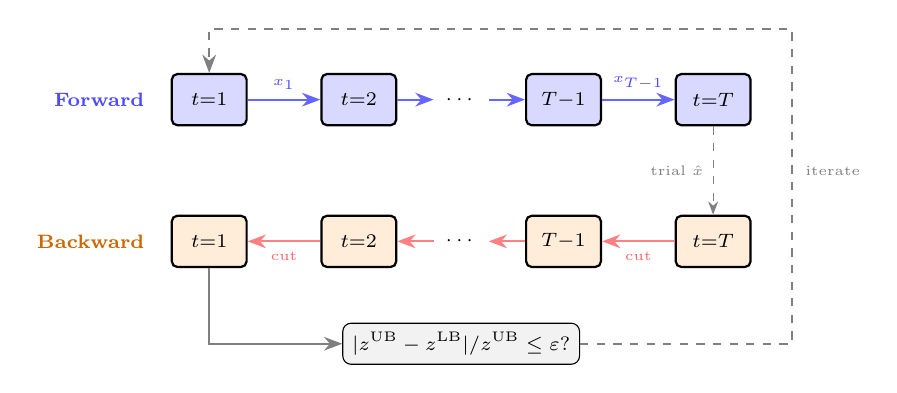
\begin{tikzpicture}[
    >=Stealth,
    stage/.style={draw, rounded corners=2pt, minimum width=0.95cm,
      minimum height=0.65cm, font=\scriptsize, thick},
    fwd/.style={stage, fill=blue!15},
    bwd/.style={stage, fill=orange!15},
    arr/.style={->, thick},
    stvar/.style={font=\tiny, blue!70},
    cutlbl/.style={font=\tiny, red!60},
  ]
    \node[font=\scriptsize\bfseries, blue!70, anchor=east] at (-0.7,1.8)
      {Forward};
    \node[font=\scriptsize\bfseries, orange!80!black, anchor=east]
      at (-0.7,0) {Backward};

    \foreach \n/\x/\l in {1/0/{t{=}1}, 2/1.9/{t{=}2}, T1/4.5/{T{-}1},
                          T/6.4/{t{=}T}} {
      \node[fwd] (f\n) at (\x,1.8) {$\l$};
      \node[bwd] (b\n) at (\x,0) {$\l$};
    }
    \node[font=\scriptsize] at (3.2,1.8) {$\cdots$};
    \node[font=\scriptsize] at (3.2,0) {$\cdots$};

    % forward: state passed to the next stage
    \draw[arr, blue!60] (f1) -- (f2) node[stvar, above, midway] {$x_1$};
    \draw[arr, blue!60] (f2) -- (2.85,1.8);
    \draw[arr, blue!60] (3.55,1.8) -- (fT1);
    \draw[arr, blue!60] (fT1) -- (fT)
      node[stvar, above, midway] {$x_{T-1}$};

    % backward: cuts passed to the previous stage
    \draw[arr, red!50] (bT) -- (bT1) node[cutlbl, below, midway] {cut};
    \draw[arr, red!50] (bT1) -- (3.55,0);
    \draw[arr, red!50] (2.85,0) -- (b2);
    \draw[arr, red!50] (b2) -- (b1) node[cutlbl, below, midway] {cut};

    % trial states handed from forward to backward pass
    \draw[->, dashed, gray, thin] (fT.south) -- (bT.north)
      node[font=\tiny, midway, left] {trial $\hat{x}$};

    % convergence check and loop
    \node[draw, rounded corners=3pt, fill=gray!10, font=\scriptsize]
      (conv) at (3.2,-1.3)
      {$|z^\text{UB} - z^\text{LB}|/z^\text{UB} \leq \varepsilon$?};
    \draw[->, thick, gray] (b1.south) |- (conv.west);
    \draw[->, thick, gray, dashed] (conv.east) -| (7.4,2.7) -| (f1.north);
    \node[font=\tiny, gray, anchor=west] at (7.45,0.9) {iterate};
  \end{tikzpicture}}%
  \caption{SDDP forward-backward iteration: the forward pass solves
    stages sequentially passing state variables (battery SoC, reservoir
    volume); the backward pass generates Benders cuts. Convergence is
    checked via the upper/lower bound gap.}
  \label{fig:sddp_flow}
\end{figure}

\subsection{Cascade Decomposition}
\label{sec:cascade}

The cascade method runs SDDP over a sequence of levels with
progressively more detailed models.  Each level defines its own LP
options (e.g.\ single bus, then the full network without losses, then
the network with losses) and SDDP options (iterations, apertures,
tolerances).  A level starts from the cuts of the previous level, kept
when their duals remain valid and otherwise re-generated, so the
expensive detailed model needs few iterations.  A typical configuration
uses 4 apertures in level~0, 8 in level~1 and the full set in level~2.
Each level may also override the solver options of its forward and
backward passes (tolerances, MIP gap, time limit, algorithm).

A level may also use its own, reduced network, produced by a network
reduction tool that merges buses and aggregates lines while keeping
every storage element.  Cuts are transferred between levels with a key
per coefficient (element class, variable and identifier) instead of a
column index, so they remain applicable when the LP is rebuilt with a
different formulation or network.  A reduced level whose network is a
relaxation of the next one (merged buses, summed inter-zonal capacities,
no Kirchhoff rows and no losses) has a cost-to-go no greater than that
of the detailed network, so its cuts are valid lower bounds and can be
kept indefinitely; cuts of a reduced level with equivalent reactances
or resistances are not guaranteed to be valid and are inherited for a
limited number of iterations.  Each level reports its bounds, gap,
iterations and aperture statistics.

\subsection{Investment Master}
\label{sec:investment_master}

For expansion problems that are too large for a monolithic LP, an
investment master in the style of OptGen chooses the investment
modules, and SDDP evaluates the expected operating cost of each plan.
Benders cuts on the investment variables return the marginal value of
each module to the master.

\subsection{One Model Across Time Scales}
\label{sec:multiscale}

Because the same element definitions are used at every scale, only the
time structure (stages and blocks of any duration) and the method change
between studies (Table~\ref{tab:scales}).

\begin{table}[t]
  \centering
  \caption{Time scales and methods}
  \label{tab:scales}
  \begin{tabular}{@{}llll@{}}
    \toprule
    Scale & Horizon & Blocks & Method \\
    \midrule
    Operation   & hours--days   & 15\,min--1\,h      & monolithic (UC) \\
    Medium term & months--years & hours, load curve & SDDP \\
    Planning    & up to 30+ yr  & representative    & SDDP, cascade, \\
                &               &                   & investment master \\
    \bottomrule
  \end{tabular}
\end{table}

The scales are coupled in two directions:
\begin{itemize}
  \item \textbf{Optimality cuts} carry water values and storage
    opportunity costs downward: the future-cost function of a planning
    or medium-term study becomes the boundary cut set of a shorter
    study, and the cascade inherits the cuts of its coarser levels.
  \item \textbf{Feasibility cuts} enforce reservoir levels and water
    rights at each scale, so the policy handed from one scale to the
    next is also feasible.
\end{itemize}

As a result, the water value used to dispatch a reservoir on a given day
is the same marginal value that the medium-term study computed for that
reservoir, and the investment plan is evaluated with the same operating
model that will later schedule it.

\paragraph{Typical periods in expansion studies.}
For expansion studies the year is usually reduced to one chronological
typical week (or a few representative days) per month, on which
storage cycles, ramps and commitment run in real time while energy,
costs and annuities are scaled to the month (Section~\ref{sec:point_stages}).
The converters provide several experimental week samplers: uniform
blocks of $H$ hours, finer blocks at the daily net-load peak and the
steepest ramps, and point samples at $N$ Chebyshev nodes with
quadrature weights.  The default window runs from Wednesday noon to
Wednesday noon, which places the weekend, where low load and high solar
drive storage cycling and curtailment, away from the cyclic closure, and
the week holding the monthly net-load peak (or the largest net energy) is
selected.  An optional refinement adds 30- or 15-minute resolution
around the sunrise and sunset ramps detected in the data: block samplers
split the base blocks there with energy-conserving, shape-preserving
cell means, and Chebyshev weeks add the nodes of the order-$2N$
Lobatto set nearest to each event, which contains the order-$N$ set,
with the weight of each dropped node split between its kept
neighbours so that all weights stay positive.  Commitment is not
refined, so the refinement adds continuous variables only.  A separate
converter, \texttt{tcheby2gtopt}, translates the validation systems of
the original Chebyshev scheduling code~\cite{matus2015chebyshev} into
both representations.

In a preliminary comparison on one expansion year of the Australian
National Electricity Market (twelve typical weeks with 138 batteries,
solved with HiGHS), the objective of the Chebyshev weeks approached the
reference with one-hour blocks from below as $N$ grew: 0.9 to 1.3\% below
it with 48 to 64 nodes and within 0.5\% with 84 nodes, against 0.24\%
for uniform two-hour blocks of the same LP size.  With 24 nodes the
week was under-resolved and lost about a third of the battery cycling.  The \texttt{cc} rule~\eqref{eq:point_cc} was closest to the
reference among the storage rules and gave the smallest LP, with the
same size as a block LP with the same number of blocks; the banded
rules add the envelope rows.  The converters therefore write
\texttt{cc} for every storage on point stages.

\subsection{Solver Backends}

All methods delegate LP/MIP solution to a plugin
(\texttt{libgtopt\_solver\_*.so}) loaded at run time.  The supported
backends are CLP/CBC~\cite{forrest2005cbc},
HiGHS~\cite{huangfu2018highs}, SCIP, NVIDIA cuOpt (GPU), CPLEX, Gurobi
and MindOpt, each declaring its capabilities (MIP, basis input and
output) to the core (Section~\ref{sec:architecture}).  Without an
explicit choice, the first available of CPLEX, HiGHS, MindOpt, CBC and
CLP is used.  Each solve reports its status and
an estimate of the condition number, and per-element variable scaling,
objective scaling and row/column equilibration (Ruiz by default for
multi-bus Kirchhoff networks, row-max otherwise) keep models with
kWh-scale batteries and TWh-scale reservoirs numerically stable.

% ============================================================================
% Section V: Software Architecture
% ============================================================================

\section{Software Architecture}
\label{sec:architecture}

\subsection{Design Principles}

The software architecture of \gtopt{} is organized around four core
principles:

\begin{enumerate}
  \item \textbf{Performance}: C++26 with cache-friendly sorted flat maps
    for sparse-matrix assembly, parallel assembly and solution of the
    (scene, phase) subproblems, and compressed in-memory LP snapshots.
  \item \textbf{Modularity}: Each power system component (generator,
    demand, line, battery, reservoir, etc.) has its own LP assembly class
    (\texttt{*\_lp.cpp}) that independently adds variables, constraints,
    and objective terms to the shared \texttt{LinearProblem}.
  \item \textbf{Extensibility}: New components and solver backends can be
    added without modifying the core LP engine.  Solver backends are
    loaded as dynamic plugins (\texttt{libgtopt\_solver\_*.so}).
  \item \textbf{Interoperability}: JSON configuration with native Apache
    Arrow/Parquet I/O enables seamless integration with Python, R, and
    other data science ecosystems.
\end{enumerate}

\subsection{System Architecture}

Fig.~\ref{fig:arch_layers} illustrates the layered architecture.

\begin{figure}[t]
  \centering
  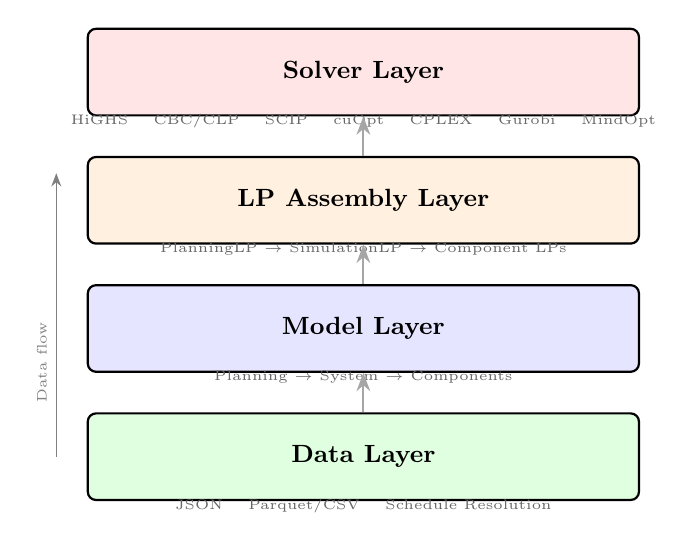
\begin{tikzpicture}[
    >=Stealth,
    layer/.style={draw, thick, rounded corners=3pt, minimum width=7cm,
      minimum height=1.1cm, font=\small, align=center},
    sublbl/.style={font=\tiny, text=black!60},
    arr/.style={->, thick, gray!70},
  ]
    % Layer 4 (bottom): Data Layer
    \node[layer, fill=green!12] (data) at (0,0)
      {\textbf{Data Layer}};
    \node[sublbl, below=-0.15cm of data]
      {JSON \quad Parquet/CSV \quad Schedule Resolution};

    % Layer 3: Model Layer
    \node[layer, fill=blue!10, above=0.5cm of data] (model)
      {\textbf{Model Layer}};
    \node[sublbl, below=-0.15cm of model]
      {Planning $\to$ System $\to$ Components};

    % Layer 2: LP Assembly Layer
    \node[layer, fill=orange!12, above=0.5cm of model] (lp)
      {\textbf{LP Assembly Layer}};
    \node[sublbl, below=-0.15cm of lp]
      {PlanningLP $\to$ SimulationLP $\to$ Component LPs};

    % Layer 1 (top): Solver Layer
    \node[layer, fill=red!10, above=0.5cm of lp] (solver)
      {\textbf{Solver Layer}};
    \node[sublbl, below=-0.15cm of solver]
      {HiGHS \quad CBC/CLP \quad SCIP \quad cuOpt \quad CPLEX \quad Gurobi \quad MindOpt};

    % Arrows between layers
    \draw[arr] (data.north) -- (model.south);
    \draw[arr] (model.north) -- (lp.south);
    \draw[arr] (lp.north) -- (solver.south);

    % Side labels
    \node[font=\tiny, rotate=90, anchor=south, gray]
      at (-3.9,1.2) {Data flow};
    \draw[->, thin, gray] (-3.9,0) -- (-3.9,3.6);
  \end{tikzpicture}
  \caption{\gtopt{} layered architecture: data ingestion, model
    construction, LP assembly, and pluggable solver backends.}
  \label{fig:arch_layers}
\end{figure}

The software is organized into four layers:

\begin{enumerate}
  \item \textbf{Data Layer}: JSON parsing (via DAW JSON Link, a
    zero-allocation header-only library), Parquet/CSV I/O (via Apache
    Arrow C++ SDK), and schedule resolution (\texttt{FieldSched<T>}
    variant type supporting scalar, vector, or filename references).
  \item \textbf{Model Layer}: The \texttt{Planning} $\rightarrow$
    \texttt{System} $\rightarrow$ component hierarchy that maps JSON
    input to C++ data structures.
  \item \textbf{LP Assembly Layer}: \texttt{PlanningLP} orchestrates
    \texttt{SimulationLP} instances (one per scenario/stage), which in
    turn assemble component LP objects (\texttt{GeneratorLP},
    \texttt{DemandLP}, \texttt{LineLP}, \texttt{BatteryLP},
    \texttt{ReservoirLP}, etc.) into a shared
    \texttt{FlatLinearProblem}.
  \item \textbf{Solver Layer}: The \texttt{SolverBackend} interface
    abstracts LP/MIP solution.  Implementations are loaded as dynamic
    plugins from configurable search paths.
\end{enumerate}

\subsection{Data Model and JSON Interface}

The input is specified as one or more JSON files containing three sections:

\begin{lstlisting}[language={},caption={Top-level JSON structure}]
{
  "options": { ... },
  "simulation": {
    "block_array": [...],
    "stage_array": [...],
    "scenario_array": [...]
  },
  "system": {
    "bus_array": [...],
    "generator_array": [...],
    "demand_array": [...],
    "line_array": [...],
    "battery_array": [...],
    ...
  }
}
\end{lstlisting}

Time-series data (demand profiles, generator capacity factors, reservoir
inflows) can be specified inline as JSON arrays, or as references to
external Parquet or CSV files in the \texttt{input\_directory}.  This
hybrid approach keeps the JSON configuration compact while supporting
arbitrarily large time-series via columnar Parquet storage.  Elements
can be referenced by name or by numeric identifier.  The command
\texttt{gtopt --json-schema} prints the JSON Schema of the input,
generated from the C++ types, for editor completion and validation.
Results are written per (scene, phase) as Parquet files (snappy or zstd)
or CSV, readable by pandas, DuckDB, Spark or Power BI.

\subsection{User Constraints: PAMPL}

Operating rules that are not part of the element library are written in
PAMPL, an AMPL-like language read from a text file.  PAMPL constraints
reference element variables by name, use parameters, sums over element
sets and scenario/stage/block domains, and can include state terms that
cross phases in SDDP.  The Chilean irrigation agreements of the Maule
and Laja basins, for example, are built from water-right elements
(Section~\ref{sec:formulation}) plus PAMPL constraints, without changes
to the C++ code.

\subsection{Auditability}

Every LP/MIP can be written as a standard LP file with readable row and
column names, and solved or checked with any external solver.  When a
run is infeasible, the LP is dumped and \texttt{gtopt\_check\_lp}
computes an irreducible infeasible subsystem.  An LP
\emph{fingerprint} records the structure of the model actually solved
(element classes, constraint families and their counts), so that
auditors and continuous integration can verify that a run uses the
intended formulation.  The complete formulation, including the SDDP
cut-validity conditions, is published with the source code.

\subsection{Python Toolchain}

A Python toolchain is provided for data preparation, conversion and
validation:

\begin{itemize}
  \item \textbf{igtopt}: Excel workbook ($\rightarrow$ JSON + Parquet)
    converter for spreadsheet-based case preparation.
  \item \textbf{Converters} from the models used in the region and in
    the literature: \texttt{plp2gtopt} (PLP, including its cuts),
    \texttt{plexos2gtopt} (PLEXOS inputs), \texttt{sddp2gtopt}
    (PSR SDDP), PSS/E, NREL Sienna, RTS-GMLC and NREL-118.
  \item \textbf{pp2gtopt / gtopt2pp}: pandapower
    ($\leftrightarrow$ gtopt) bidirectional converters for power flow
    model exchange.
  \item \textbf{gtopt\_compare}: Automated cross-validation against
    pandapower DC OPF on IEEE test networks.
  \item \textbf{gtopt\_diagram}: network and hydro-topology diagrams.
  \item \textbf{gtopt-net}: network reduction for long-term studies,
    with decisions mapped back onto the full network.
  \item \textbf{run\_gtopt / gtopt\_monitor}: execution management with
    a terminal dashboard and live SDDP convergence monitoring.
  \item \textbf{Validation tools}: \texttt{gtopt\_check\_json},
    \texttt{gtopt\_check\_lp}, \texttt{gtopt\_check\_output},
    \texttt{gtopt\_check\_solvers} for input validation and diagnostics.
\end{itemize}

\subsection{Web and GUI Services}

Two companion services provide graphical interfaces:

\begin{itemize}
  \item \textbf{webservice}: a Next.js REST API and browser UI for
    submitting optimization jobs, monitoring progress and browsing
    results.
  \item \textbf{guiservice}: a Python/Flask application for creating
    and editing cases, viewing the network topology and plotting
    results in the browser.
\end{itemize}

\subsection{Engineering Practice}

The C++ library, the Python tools and the web services are covered by
unit and integration test suites (more than 5\,000 C++ test cases),
static analysis (clang-tidy and CodeQL) and coverage measurement, all
run in continuous integration on every change.  The test suite includes
the benchmark cases of Section~\ref{sec:validation}, reference results
for each case, and solver-specific tolerances where backends may return
different optimal dual vertices.

% ============================================================================
% Section VI: Validation and Benchmark Results
% ============================================================================

\section{Validation and Benchmark Results}
\label{sec:validation}

\gtopt{} is validated on IEEE benchmark networks and derived cases,
on published SDDP, unit-commitment, reserve and gas-network benchmarks,
and against independent models of the same problems.  All IEEE test
cases converge to optimal solutions (status~0) with zero optimality
gap; Table~\ref{tab:benchmarks} summarizes them.

\begin{table*}[t]
  \centering
  \caption{IEEE Benchmark Results (scale\_objective = 1000, CLP solver)}
  \label{tab:benchmarks}
  \begin{tabular}{@{}llcccccrc@{}}
    \toprule
    \textbf{Case} & \textbf{Type} & \textbf{Buses} & \textbf{Gen}
      & \textbf{Dem} & \textbf{Lines} & \textbf{Bat}
      & \textbf{Obj (scaled)} & \textbf{Blocks} \\
    \midrule
    \multicolumn{9}{@{}l}{\textit{Standard IEEE DC OPF (single snapshot)}} \\
    \texttt{ieee\_4b\_ori}   & DC OPF     & 4  & 2 & 2  & 5  & -- & 5.000    & 1  \\
    \texttt{ieee\_9b\_ori}   & DC OPF     & 9  & 3 & 3  & 9  & -- & 55.184   & 1  \\
    \texttt{ieee\_14b\_ori}  & DC OPF     & 14 & 5 & 11 & 20 & -- & 8.334    & 1  \\
    \texttt{ieee30b}          & DC OPF     & 30 & 6 & 21 & 41 & -- & 5.668    & 1  \\
    \texttt{ieee\_57b}       & DC OPF     & 57 & 7 & 42 & 80 & -- & 25.016   & 1  \\
    \midrule
    \multicolumn{9}{@{}l}{\textit{24-hour dispatch with solar profiles}} \\
    \texttt{ieee\_9b}        & Solar+OPF  & 9  & 3 & 3  & 9  & -- & 5400.007 & 24 \\
    \texttt{ieee\_14b}       & Solar+OPF  & 14 & 5 & 11 & 20 & -- & 1492.283 & 24 \\
    \midrule
    \multicolumn{9}{@{}l}{\textit{Battery energy storage}} \\
    \texttt{bat\_4b}         & BESS+OPF   & 4  & 3 & 2  & 5  & 1  & 14.160   & 4  \\
    \texttt{bat\_4b\_24}     & BESS+OPF   & 4  & 3 & 2  & 5  & 1  & 44.862   & 24 \\
    \midrule
    \multicolumn{9}{@{}l}{\textit{Capacity expansion}} \\
    \texttt{exp\_gen\_4b}    & Gen. exp.  & 4  & 2 & 2  & 5  & -- & 5.029    & 4  \\
    \texttt{exp\_bat\_4b}    & Bat. exp.  & 4  & 3 & 2  & 5  & 1  & 12.437   & 4  \\
    \texttt{c0}              & Dem. exp.  & 1  & 1 & 1  & 0  & -- & 23.163   & 5 stages \\
    \bottomrule
  \end{tabular}
\end{table*}

\subsection{Test Systems and Data Sources}
\label{sec:test_systems}

Table~\ref{tab:test_systems} lists the public test systems included in
the repository (directory \texttt{cases/}) or read by its converters,
with their sources.  Each case in the repository carries reference
results that are checked in continuous integration.  The standard test
systems, the example systems of other tools and the published case
studies are also distributed, converted with the converters of
\gtopt{}, in the companion case repository~\cite{gtoptcases}, whose
benchmark collection keeps the upstream files of openly licensed data
and, for data without a licence, a recipe that downloads a pinned,
checksum-verified copy and converts it locally.

\begin{table*}[t]
  \centering
  \caption{Public test systems used for validation and their sources}
  \label{tab:test_systems}
  \small
  \setlength{\tabcolsep}{4pt}
  \begin{tabular}{@{}llll@{}}
    \toprule
    \textbf{System} & \textbf{Size} & \textbf{Used for} & \textbf{Source} \\
    \midrule
    IEEE 4-bus and battery variants & 4 buses & DC OPF, storage, expansion & illustrative \\
    Anderson--Fouad 9-bus & 9 buses & DC OPF, solar profile & \cite{anderson2002power} \\
    IEEE 14-, 30-, 57-bus & 14--57 buses & DC OPF, pandapower cross-check & \cite{pstca, ieee30bus, ieee57bus, thurner2018pandapower} \\
    IEEE 118-bus & 118 buses & DC OPF & \cite{pstca, pglibopf2019} \\
    PGLib-OPF v23.07 (5 to 300 buses) & 5--300 buses & DC OPF & \cite{pglibopf2019} \\
    IEEE RTS-96 (24-bus) & 24 buses & unit commitment with OPF & \cite{grigg1999rts96, pglibopf2019} \\
    RTS-GMLC & 73 buses & UC and dispatch with renewables & \cite{barrows2020rtsgmlc} \\
    NREL-118 & 118 buses & one-week hourly dispatch & \cite{pena2018nrel118, powersimulations} \\
    NREL Sienna test systems & 1--5 buses & UC, hydro, storage, reserves & \cite{lara2021powersystems, powersimulations} \\
    UnitCommitment.jl fixtures & 14--118 buses & UC MIP vs.\ UnitCommitment.jl & \cite{xavier2024ucjl} \\
    Clustered-UC case studies & 39, 118 buses & UC MIP vs.\ published model & \cite{morales2019cuc, cucdata} \\
    Power-based UC example & 1 bus & published schedule and cost & \cite{philipsen2019trading} \\
    Chebyshev scheduling systems & 1--9 buses & block vs.\ point-sampled stages & \cite{matus2015chebyshev} \\
    Non-convex pricing examples & 1--3 buses & UC prices, uplift & \cite{oneill2005pricing, gribik2007convexhull, hua2017convexhull} \\
    MATPOWER \texttt{case30} reserves & 30 buses & zonal reserves, interfaces & \cite{matpower_case30} \\
    Badesa et al.\ frequency services & 1 bus & reserve and inertia prices & \cite{badesa2020pricing} \\
    Polish \texttt{case3375wp} (R.~Korab) & 3\,375 buses & large-network DC OPF & \cite{zimmerman2011matpower} \\
    SDDP.jl examples (first steps, hydro valleys, FAST) & 1--2 reservoirs & SDDP vs.\ published bounds & \cite{dowson2020sddp_jl, cambier_fast} \\
    PSR SDDP sample cases & multi-system & \texttt{sddp2gtopt} hydrothermal & \cite{psrclasses} \\
    Saldarriaga pipe chain & 4 gas nodes & Weymouth pressures & \cite{saldarriaga2018phd} \\
    GasLib-11 & 11 gas nodes & radial gas network & \cite{schmidt2017gaslib, pfetsch2015nominations} \\
    Belgian network (GasModels \texttt{A1}) & 24 gas nodes & radial gas network & \cite{dewolf2000gas, gasmodels} \\
    GasModels \texttt{case-6} & 6 gas nodes & exact Weymouth, meshed SLP & \cite{gasmodels} \\
    Hu--Ryan 6-bus/7-node, IEEE-24/Belgian-20 & 6--24 buses, 7--20 gas nodes & coupled gas--power & \cite{hu2019data, hu2019stochastic} \\
    Ratha et al.\ 24-bus/12-node & 24 buses, 12 gas nodes & meshed coupled gas--power & \cite{ratha2020data, ratha2020affine, ordoudis2019gas} \\
    CEN daily schedules (PLEXOS) & $\sim$250 buses & vs.\ official schedule & \cite{cen_pcp}, Section~\ref{sec:cases} \\
    Real systems of six countries & 3--3\,374 buses & UC, SDDP, OPF & Section~\ref{sec:gtopt_cases} \\
    \bottomrule
  \end{tabular}
\end{table*}

\subsection{Public Real-System Cases}
\label{sec:gtopt_cases}

Beyond the benchmark networks of Table~\ref{tab:test_systems}, GTOpt
is exercised on real power systems through the public companion
repository \texttt{gtopt-cases}~\cite{gtoptcases2026}.  Each case is
built with the GTOpt converters from data published by a system
operator, market operator or regulator, and is distributed with its
source data, the converted case, the exact command to run and rebuild
it, and the provenance (converter revision, flags and file hashes).
Only inputs are published, so that results can be reproduced and
compared independently; the cases are provided as is and are not
validated by the publishing institutions, which keep all rights over
the data.  Table~\ref{tab:gtopt_cases} lists the six countries
covered.  The Irish data may not be redistributed, so that case is
published as a recipe that downloads the public files and converts
them locally.  The 23-year Chilean cases are committed for their first
year to limit the repository size; the full horizon is built from the
same sources with one converter command.

\begin{table*}[t]
  \centering
  \caption{Real-system cases in \texttt{gtopt-cases}}
  \label{tab:gtopt_cases}
  \small
  \begin{tabular}{@{}lllll@{}}
    \toprule
    \textbf{Country} & \textbf{System · publisher} & \textbf{Cases} & \textbf{Horizon} & \textbf{Converter} \\
    \midrule
    Australia & NEM · AEMO & 1 dispatch, 2026 ISP model (Step Change) & 1 week, hourly & \texttt{plexos2gtopt} \\
    Chile & SEN · CEN & 14 daily operation programmes (unit commitment) & 1 week each & \texttt{plexos2gtopt} \\
          &            & 3 hydrothermal SDDP (PLP), irrigation agreements & 2, 4.5 and 23 years & \texttt{plp2gtopt} \\
          &            & 3 PET 2027 transmission planning bases (PLP) & 23 years & \texttt{plp2gtopt} \\
    Guatemala & SNI · AMM, EOR & 2 NCP daily/weekly dispatches & 1 week & \texttt{sddp2gtopt} \\
              &                & 6 PSS\textregistered E network snapshots & 1 hour & \texttt{psse2gtopt} \\
              &                & 6 annual SDDP programmes & 1 year & \texttt{sddp2gtopt} \\
    Ireland & SEM · SEM Committee (CRU, UR) & 1 unit commitment (recipe only) & 1 week, hourly & \texttt{plexos2gtopt} \\
    Peru & SEIN · COES & 4 SDDP cases, 2026--2029 reserve-margin study & 1 year each & \texttt{sddp2gtopt} \\
    Poland & MATPOWER \texttt{case3375wp} & 1 DC OPF, 3\,374 buses & 1 hour & \texttt{pp2gtopt} \\
    \bottomrule
  \end{tabular}
\end{table*}

\subsection{IEEE 4-Bus Network}
\label{sec:ieee4b}

The IEEE 4-bus test case consists of a fully meshed network with 4 buses
and 5 transmission lines (Fig.~\ref{fig:ieee4b}).  Two generators
(g1: 300~MW at \$20/MWh, g2: 200~MW at \$35/MWh) supply two demands
(d3: 150~MW, d4: 100~MW).

\begin{figure}[t]
  \centering
  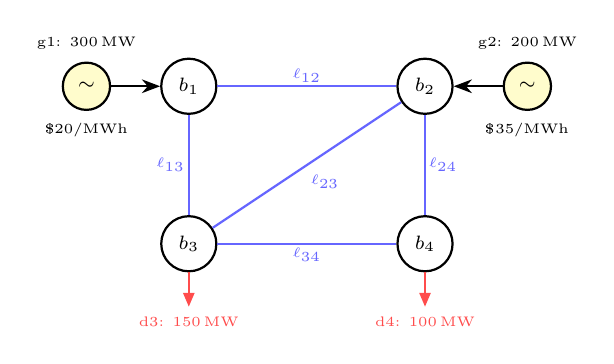
\begin{tikzpicture}[
    >=Stealth,
    bus/.style={circle, draw, thick, fill=white, minimum size=0.7cm,
      font=\scriptsize\bfseries},
    genbox/.style={circle, draw, thick, fill=yellow!20,
      minimum size=0.6cm, font=\scriptsize},
    dembox/.style={-{Triangle[length=5pt,width=4pt]}, thick, red!70},
    line/.style={thick, blue!60},
    linelab/.style={font=\tiny, fill=white, inner sep=1pt},
  ]
    % Buses in diamond layout
    \node[bus] (b1) at (0,2)   {$b_1$};
    \node[bus] (b2) at (3,2)   {$b_2$};
    \node[bus] (b3) at (0,0)   {$b_3$};
    \node[bus] (b4) at (3,0)   {$b_4$};

    % Generators
    \node[genbox] (g1) at (-1.3,2) {$\sim$};
    \node[font=\tiny, above=1pt of g1] {g1: 300\,MW};
    \node[font=\tiny, below=1pt of g1] {\$20/MWh};
    \draw[->, thick] (g1) -- (b1);

    \node[genbox] (g2) at (4.3,2) {$\sim$};
    \node[font=\tiny, above=1pt of g2] {g2: 200\,MW};
    \node[font=\tiny, below=1pt of g2] {\$35/MWh};
    \draw[->, thick] (g2) -- (b2);

    % Demands (downward arrows from buses)
    \draw[dembox] (b3) -- ++(0,-0.8)
      node[below, font=\tiny] {d3: 150\,MW};
    \draw[dembox] (b4) -- ++(0,-0.8)
      node[below, font=\tiny] {d4: 100\,MW};

    % Transmission lines
    \draw[line] (b1) -- (b2) node[linelab, midway, above] {$\ell_{12}$};
    \draw[line] (b1) -- (b3) node[linelab, midway, left]  {$\ell_{13}$};
    \draw[line] (b2) -- (b3) node[linelab, pos=0.5, below right=2pt and 0pt]
      {$\ell_{23}$};
    \draw[line] (b2) -- (b4) node[linelab, midway, right] {$\ell_{24}$};
    \draw[line] (b3) -- (b4) node[linelab, midway, below] {$\ell_{34}$};
  \end{tikzpicture}
  \caption{IEEE 4-bus network: 2 generators, 2 demands, 5 lines forming
    a fully meshed topology for DC OPF validation.}
  \label{fig:ieee4b}
\end{figure}

Under DC OPF with Kirchhoff constraints, the cheaper generator g1
dispatches 250~MW and g2 idles.  The scaled objective value is
$5.0 = 250 \times 20 / 1000$.  Power routes through parallel paths
(b1$\rightarrow$b3 and b1$\rightarrow$b2$\rightarrow$b3) according to
the relative reactances.

\subsection{IEEE 9-Bus Network}
\label{sec:ieee9b}

The Anderson--Fouad 9-bus system~\cite{anderson2002power} has three
generation areas connected by a meshed transmission network
(Fig.~\ref{fig:ieee9b}).  Generators g1 (250~MW, \$20/MWh),
g2 (300~MW, \$35/MWh), and g3 (270~MW, \$30/MWh) serve demands at
buses 5, 7, and~9 (total 315~MW).

\begin{figure}[t]
  \centering
  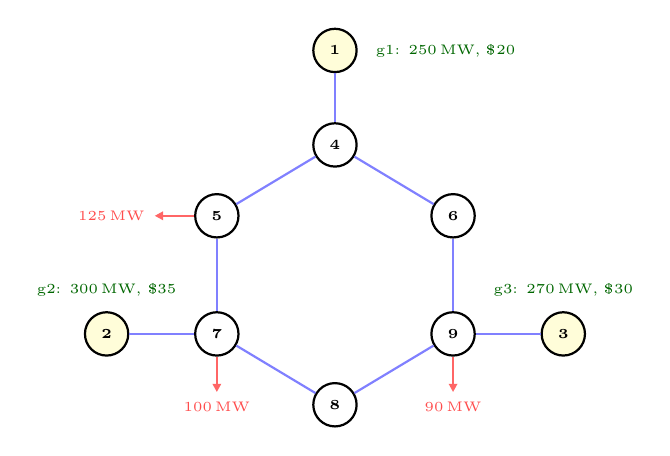
\begin{tikzpicture}[
    >=Stealth,
    bus/.style={circle, draw, thick, fill=white, minimum size=0.55cm,
      font=\tiny\bfseries, inner sep=1pt},
    genbus/.style={bus, fill=yellow!15},
    demlab/.style={font=\tiny, red!70},
    genlab/.style={font=\tiny, green!40!black},
    line/.style={thick, blue!50},
    dem/.style={-{Triangle[length=3pt,width=3pt]}, thick, red!60},
  ]
    % network ring 4-5-7-8-9-6-4, generator buses 1, 2, 3 outside
    \node[bus] (b4) at (0,1.9)     {4};
    \node[bus] (b5) at (-1.5,1.0)  {5};
    \node[bus] (b6) at (1.5,1.0)   {6};
    \node[bus] (b7) at (-1.5,-0.5) {7};
    \node[bus] (b9) at (1.5,-0.5)  {9};
    \node[bus] (b8) at (0,-1.4)    {8};
    \node[genbus] (b1) at (0,3.1)    {1};
    \node[genbus] (b2) at (-2.9,-0.5) {2};
    \node[genbus] (b3) at (2.9,-0.5)  {3};

    \foreach \a/\b in {1/4, 4/5, 4/6, 5/7, 6/9, 7/8, 8/9, 2/7, 3/9}
      \draw[line] (b\a) -- (b\b);

    \node[genlab, right=3pt of b1] {g1: 250\,MW, \$20};
    \node[genlab, above=2pt of b2] {g2: 300\,MW, \$35};
    \node[genlab, above=2pt of b3] {g3: 270\,MW, \$30};

    \draw[dem] (b5.west) -- ++(-0.5,0) node[demlab, left] {125\,MW};
    \draw[dem] (b7.south) -- ++(0,-0.45) node[demlab, below] {100\,MW};
    \draw[dem] (b9.south) -- ++(0,-0.45) node[demlab, below] {90\,MW};
  \end{tikzpicture}
  \caption{IEEE 9-bus network: three generation areas (buses 1--3)
    serve three demands (buses 5, 7, 9) through a meshed
    9-line transmission network.}
  \label{fig:ieee9b}
\end{figure}

In the single-snapshot case (\texttt{ieee\_9b\_ori}), economic dispatch
follows merit order constrained by network topology.  The 24-hour variant
(\texttt{ieee\_9b}) replaces g3 with a solar plant (\$0/MWh) whose output
follows a daily capacity profile peaking at noon.  During daylight hours,
zero-cost solar generation displaces g2; at night, g2 carries the load.

\subsection{IEEE 14-Bus Network}
\label{sec:ieee14b}

The 14-bus system has 5 generators, 11 demands, and 20 transmission lines.
The constrained variant (\texttt{ieee\_14b}) tightens limits on lines
$\ell_{1-2}$ and $\ell_{1-5}$, forcing both to saturate simultaneously
at the evening demand peak.  This validates that shadow prices (Lagrange
multipliers of the binding Kirchhoff constraints) are computed correctly.

\subsection{IEEE 30-Bus and 57-Bus Networks}

The 30-bus~\cite{ieee30bus} and 57-bus~\cite{ieee57bus} systems test
scalability.  The 30-bus case has 6 generators, 21 demands, and 41 lines;
the 57-bus case has 7 generators, 42 demands, and 80 lines.  Both
converge to optimal solutions in under one second with the CLP solver.

\subsection{Battery Storage Cases}
\label{sec:bat_cases}

The \texttt{bat\_4b} case augments the 4-bus network with a 200~MWh
battery at bus~3 (60~MW charge/discharge, 95\% round-trip efficiency) and
a solar generator with a 4-period capacity profile.  The battery charges
during solar peak and discharges during evening demand, reducing total
system cost compared to the no-storage baseline.

The 24-hour variant (\texttt{bat\_4b\_24}) demonstrates full daily
charge/discharge cycling with state-of-charge tracking across all
24~blocks.

\subsection{Capacity Expansion Cases}
\label{sec:exp_cases}

Three expansion cases validate the investment planning formulation:

\begin{itemize}
  \item \texttt{exp\_gen\_4b}: Generator g1 can be expanded by up to
    290~MW at \$1000/year annualized cost.  The optimizer adds capacity
    to avoid dispatching expensive g2.
  \item \texttt{exp\_bat\_4b}: Battery expansion with 200~MWh modules
    at \$1000/year.  The optimizer installs storage to arbitrage
    solar/thermal cost differentials.
  \item \texttt{c0}: Multi-stage demand expansion (5 stages, 10\%
    discount rate).  Demand grows through 20~MW modules at
    \$8760/year.  The optimizer balances discounted investment cost
    against increasing served demand.
\end{itemize}

\subsection{Cross-Validation with pandapower}

The \texttt{gtopt\_compare} tool performs automated cross-validation
against pandapower~\cite{thurner2018pandapower} DC OPF on all IEEE test
networks (4, 9, 14, 30, 57 buses).  For each case, both tools solve the
same network data and compare:

\begin{itemize}
  \item Objective function value (total generation cost)
  \item Generator dispatch (MW per generator)
  \item Bus angles (radians)
  \item Line flows (MW)
  \item Locational marginal prices (bus balance duals)
\end{itemize}

Results match to within solver tolerance ($<10^{-6}$ relative error)
for all standard IEEE cases, confirming the correctness of the DC OPF
implementation in \gtopt{}.

\subsection{SDDP Against Published Benchmarks}
\label{sec:sddp_bench}

The SDDP implementation is checked in continuous integration against
published reference values:
\begin{itemize}
  \item \textbf{SDDP.jl \emph{first steps}}~\cite{dowson2020sddp_jl}: a
    three-stage hydrothermal problem with stagewise-independent inflows
    and a published lower bound of 8333.33, confirmed in-repo by the
    27-leaf extensive form.  Every iterate of \gtopt{} is a valid lower
    bound and the sequence is monotone.  With the default aperture
    backward pass it converges to 8055.6, 3.3\% below the exact value,
    because the cuts are built from the resampled apertures rather than
    from the exact expectation.  Depending on the dual vertex returned
    by the LP solver, it can also reach the exact value.
  \item \textbf{SDDP.jl \emph{Markov uncertainty}} and
    \emph{generation expansion}: checked against extensive-form and
    MIP oracles.
  \item \textbf{Infanger--Morton dual sharing}~\cite{infanger1996cutsharing}:
    cut-for-cut agreement
    of the shared-dual backward pass with the standard one where the
    theory guarantees it.
\end{itemize}

In addition, the equivalence between the monolithic LP and SDDP is
tested on multi-stage cases: with the same data, the converged SDDP
bounds match the monolithic optimum within the convergence tolerance.
The water value of a spilling reservoir is also checked against
hand-derived values, with free and priced exits, in monolithic and
SDDP runs.

\subsection{Unit-Commitment and Reserve Benchmarks}
\label{sec:uc_bench}

The commitment, reserve and pricing models of
Section~\ref{sec:formulation} are cross-checked against other
implementations and against published values:
\begin{itemize}
  \item \textbf{UnitCommitment.jl}~\cite{xavier2024ucjl}: its IEEE
    14-bus and 118-bus test fixtures (tiered startup costs, minimum
    up/down times, ramps, initial conditions, profiled renewables) are
    converted to \gtopt{} and solved as MIPs; the hourly commitment
    and dispatch are compared with the solution of UnitCommitment.jl
    on the same instance, with the full network and with a copper
    plate.
  \item \textbf{NREL Sienna}~\cite{lara2021powersystems,
    powersimulations}: the PowerSimulations.jl test systems of the
    5-bus PJM network (cascaded hydro, pumped storage, an HVDC link, an
    interruptible load, a single monitored line, time-varying fuel
    prices, a battery) are compared on hourly and aggregate dispatch,
    and its reserve systems (range reserves and operating-reserve
    demand curves, represented as stacked priced reserve zones) on the
    objective to a relative $10^{-6}$ and on the hourly reserve totals.
  \item \textbf{Clustered unit commitment}~\cite{morales2019cuc}: the
    modified IEEE 39-bus and 118-bus systems of Morales-Espa\~na and
    Tejada-Arango, built from the published data~\cite{cucdata} as
    individual-unit commitment problems.  An independent transcription
    of the published model reaches the same incumbents as \gtopt{} to
    the cent.  The objectives reported in the paper are higher by
    $0.8\%$ to $2.6\%$ over its four cases, by an amount that grows
    with the reserve requirement and, for the 39-bus system, vanishes
    when extrapolated to zero reserve; this points to a different
    reserve representation in the code behind the published table.  The
    block formulation of Section~\ref{sec:sc}, applied to the same hours
    as one non-chronological stage, is checked to remain a relaxation of
    the chronological commitment.
  \item \textbf{Power-based commitment}: the day-ahead example of
    Philipsen et al.~\cite{philipsen2019trading} (two ramp-limited
    units, seven hours) is solved with the formulation of
    Section~\ref{sec:pbuc}; the published power-based cost and the
    boundary powers of both units are reproduced exactly, and the
    energy-block formulation reproduces the lower energy-based cost of
    the same paper, which the ramp limits cannot actually deliver.
  \item \textbf{Point-sampled stages}: small hydrothermal, battery,
    network, commitment and periodic cases, each in an hourly-block and
    a Chebyshev--Lobatto point version, are converted from the
    validation systems of the Chebyshev scheduling
    code~\cite{matus2015chebyshev}; their objectives are checked
    against hand-derived or closed-form values and as regressions, and
    the storage of every rule is checked to be conserved over a closed
    period.
  \item \textbf{Non-convex pricing}: the fixed, relaxed and fast-start
    pricing modes reproduce the prices and uplifts of the published
    examples of O'Neill et al.~\cite{oneill2005pricing}, Gribik, Hogan
    and Pope~\cite{gribik2007convexhull} and Hua and
    Baldick~\cite{hua2017convexhull}; the remaining differences are
    explained by dual degeneracy or by ramp-coupled relaxations that are
    not the convex hull.
  \item \textbf{Reserves}: the MATPOWER zonal-reserve
    case~\cite{matpower_case30} (two overlapping zones and interface
    limits) is reproduced exactly, including the zone prices and the
    reserve cost, and so are the economic-dispatch tables of Badesa et
    al.~\cite{badesa2020pricing} for energy and frequency-response
    prices.
  \item \textbf{Emissions}: the coal--gas dispatch of the
    myopic-pathway example of PyPSA~\cite{brown2018pypsa}, reduced to
    one period with a CO$_2$ cap, and a three-zone combined-cycle
    system with the technology parameters of the three-zone example of
    GenX~\cite{jenkins2017genx} are solved with a binding cap; the
    dispatch and the carbon price (the dual of the cap) are checked
    against hand-derived solutions.
\end{itemize}

\subsection{Natural-Gas Network Benchmarks}
\label{sec:gas_bench}

The gas network of Section~\ref{sec:gas} is checked in continuous
integration on the cases of Table~\ref{tab:gas_bench}.  Each reference
comes either from a published value or from an independent model built
outside \gtopt{}: an LP of the same tangent formulation (SciPy with
HiGHS~\cite{huangfu2018highs}) or an exact nonlinear Weymouth solve.
The coupled cases are LP reductions of the published data (unit
commitment relaxed, deterministic wind, gas storage as a capped
supply), so their objectives are not comparable with the published
stochastic results.

\begin{table*}[t]
  \centering
  \caption{Gas network benchmarks: what each case validates and its
    reference (objective in the case's own units)}
  \label{tab:gas_bench}
  \small
  \begin{tabular}{@{}p{3.3cm}p{6.2cm}p{6.6cm}@{}}
    \toprule
    \textbf{Case} & \textbf{Validates} & \textbf{Reference} \\
    \midrule
    Saldarriaga Fig.~2.2(b)~\cite{saldarriaga2018phd}
      & three pipes in series, 32 tangents
      & published node pressures 90/70/50/30~bar within the tangent
        bound (0.05~bar); objective of the independent LP \\
    GasLib-11, valve closed~\cite{schmidt2017gaslib}
      & radial network with compressors
      & independent LP (295.41); exact Weymouth drop on the LP flows \\
    Belgian \texttt{A1}~\cite{dewolf2000gas, gasmodels}
      & 19 pipes and 4 stations after merging parallel arcs
      & independent LP (8849.43); shedding only at the node whose
        pressure floor cannot be met \\
    GasModels \texttt{case-6}~\cite{gasmodels}
      & loop with fixed orientation and 64 tangents; the same loop with
        linearized pipes and SLP
      & published exact optimum $-253.683$: the tangent LP is within
        $1.6\cdot10^{-5}$ (relative); the SLP matches the exact NLP to
        $10^{-5}$ \\
    Hu--Ryan 6-bus/7-node~\cite{hu2019data}
      & coupled radial system, 24~h
      & independent LP; the exact Weymouth optimum is 0.68\% higher
        because an upper pressure bound downstream binds, which the
        exactness report flags on that pipe \\
    Hu--Ryan IEEE-24/Belgian-20~\cite{hu2019data}
      & coupled system, radial and SLP variants
      & radial tangent LP within 0.0099\% of the exact optimum; the SLP
        variant reaches the exact optimum \\
    Ratha et al.\ 24-bus/12-node~\cite{ratha2020data}, system
      of~\cite{ordoudis2019gas, ordoudis2018data}
      & meshed coupled system, gas SLP, compressors as ratio-bounded
        stations
      & independent SLP, unchanged by a polish on the exact NLP, i.e.\
        a local optimum of the exact problem \\
    Elevation chain
      & 0--2000--4000~m chain, term~\eqref{eq:gas_elevation}
      & closed-form outlet pressures (56.747 and 44.673~bar) \\
    Component cases
      & compressor fuel models and drives, line pack, plant pressure
        gate, booster and derate
      & independent LP of each variant: objective to $10^{-5}$
        (relative), pressures to 0.01~bar \\
    \bottomrule
  \end{tabular}
\end{table*}

The unit tests additionally check the Weymouth constant and the
line-pack coefficient, the tangent envelope against the exact curve,
the compressor-fuel planes against analytic derivatives, the
convergence of the SLP on loops, under flow reversal and on degenerate
splits, and the replay of the re-linearised rows when LP snapshots are
compressed.

\paragraph{Stylised Chilean studies.}
The gas elements were also applied to stylised studies of the central
Chilean network, in which LNG is regasified at the coast, piped to the
capital region and delivered to combined-cycle plants whose turbines
need a minimum fuel-gas pressure.  These studies explore the interaction
between the minimum plant pressure, a compressor station on the trunk,
an on-site fuel-gas booster, pressure derating and multi-day line pack,
and they cross-check the native elements against an earlier formulation
of the same LP built from generic user-defined variables and
constraints.  The data are plausible values chosen for the study, not
the parameters of the actual pipelines or plants.  Pipelines that cross
the Andes, as in the north of the country, motivated the elevation
term, which changes the attainable delivery pressure substantially on
such routes.

\subsection{Real Systems}
\label{sec:real_systems}

The companion case repository~\cite{gtoptcases} also publishes the
inputs of real systems converted from the public data of their system
operators and regulators, together with the instructions to run them:
daily schedules, medium- and long-term SDDP cases and a transmission
planning case of the Chilean system~\cite{cen_pcp}; daily, weekly and
long-term cases of Guatemala~\cite{amm_eor}; SDDP cases of
Peru~\cite{coes_mrfo}; production-cost and monthly expansion cases of
the Australian National Electricity Market from the 2026 Integrated
System Plan~\cite{aemo2026isp}; unit-commitment weeks of the Irish
Single Electricity Market~\cite{sem2025plexos}; and the Polish
3\,375-bus network~\cite{zimmerman2011matpower}.  The data remain the
property of their publishers; source files are redistributed only where
their terms allow, and otherwise fetched from the publisher.  These
cases exercise the converters from PLEXOS, PLP, PSR SDDP and PSS/E at
national scale; the comparison of Section~\ref{sec:cases} uses the
Chilean daily schedules.

% ============================================================================
% Section VII: Comparison with the Chilean daily schedule (CEN / PLEXOS)
% ============================================================================

\section{Comparison with the Chilean Daily Schedule}
\label{sec:cases}

The Chilean system operator, the Coordinador El\'ectrico Nacional (CEN),
computes the daily operation schedule of the national system (SEN) with
PLEXOS.  For each schedule, the input data and the solution (dispatch,
line flows, losses and marginal costs per bus and hour) are available.
This makes it possible to compare an independent model against the
official one on the full national network.

\subsection{Setup}

The comparison uses the CEN schedules of 14 days between October~2025
and May~2026,
plus additional days for specific checks.  Each case has a horizon of
seven days at hourly resolution, with about 250 buses and 315 lines,
hydro cascades, batteries, unit commitment and reserves.  The PLEXOS
inputs are converted with \texttt{plexos2gtopt} in a mode that follows
the PLEXOS conventions as closely as possible, and solved by \gtopt{}
with the monolithic method (MIP gap 0.5\%).  The first day
of each horizon, which is the day actually scheduled, is compared bus
by bus and hour by hour.  The comparison covers results only, not computing times.

The CEN has used two loss models: a piecewise-linear model (in 2021) and
a generalized, single-pass loss model in the recent schedules.  \gtopt{}
is run with two of the models of Section~\ref{sec:losses}:
\begin{itemize}
  \item \textbf{piecewise}: the traditional piecewise model with free
    losses ($\varepsilon_\ell = 0$);
  \item \textbf{tangent}: the tangent outer approximation with a loss
    price $\varepsilon_\ell = 1$~\$/MWh.
\end{itemize}

\subsection{Losses}

Table~\ref{tab:cen_losses} compares the losses of the LP with the
physical losses $R_\ell f_\ell^2/V_\ell^2$ evaluated at the LP flows,
over the seven-day horizon of the 14 cases.  With free piecewise losses,
the LP losses are 2.5 times the physical value in the median case.  The
excess comes from the fictitious-sink mechanism of
Section~\ref{sec:losses}: filling expensive segments first and
circulating flow in both directions when the sum of the two end-bus
duals is negative.  On the week of 7~April~2026, for example, the
piecewise model loses 91~GWh more than the physical losses, 65~GWh of
them in hours with $\pi_{a_\ell}+\pi_{b_\ell}<0$; the tangent model
loses 6~GWh more, and spills the surplus renewable energy instead.

\begin{table}[t]
  \centering
  \caption{LP losses versus physical losses over the horizon
    (median and range over 14 cases)}
  \label{tab:cen_losses}
  \begin{tabular}{@{}lcc@{}}
    \toprule
    & Piecewise, free & Tangent, $\varepsilon{=}1$ \\
    \midrule
    LP / physical losses & 2.50 (1.05--3.78) & 1.03 (1.00--1.19) \\
    Excess over physical & 152\% & 5\% \\
    \bottomrule
  \end{tabular}
\end{table}

The CEN's own solutions show the same trade-off.  In the two 2021
schedules solved with the piecewise model, the PLEXOS losses during the
hours with zero marginal cost are five times the secant approximation.
The fictitious losses amount to 8.7 and 16.1~GWh, i.e.\ 4.9\% and 8.6\%
of the daily demand, and the prices stay at exactly zero, never
negative.  In the recent schedules, solved with the generalized loss
model, the fictitious losses disappear but the surplus has no sink
left.  Marginal costs then become negative: in most of these schedules,
slightly negative across the whole system during solar hours, and on
one day down to $-132$~\$/MWh in a congested pocket of the northern
grid.  Under surplus, a loss model therefore faces a dilemma: either
fictitious losses with zero prices, or physical losses with negative
prices.  The tangent model with a small loss price chooses the latter,
consistently with the CEN's current practice.

\subsection{Marginal Costs}

The first comparison of marginal costs showed a moderate agreement
(median correlation 0.39 and mean absolute error 21~\$/MWh over all
buses, 11~\$/MWh at the reference bus, Polpaico~220~kV).  Its largest
deviations were deeply negative prices at a small load bus in the north,
down to $-891$~\$/MWh, where PLEXOS never goes below
$-1.3$~\$/MWh.  Inspecting the LP traced them to the conversion of 173
lines whose limits PLEXOS does not enforce: PLEXOS operates some of
them well above their rating (e.g.\ 190~MW on a 100~MW transformer),
whereas the converter had kept the rating as a hard limit.  The
congested chain created an isolated pocket with negative prices.
Converting these lines as PLEXOS treats them (free up to three times the
rating, penalized up to six times) removes the artifact
(Table~\ref{tab:cen_cmg}).

\begin{table}[t]
  \centering
  \caption{Hourly marginal costs of day~1, \gtopt{} vs.\ PLEXOS (CEN),
    piecewise losses: correlation and mean absolute error [\$/MWh] over
    all buses, with unenforced lines as hard limits (strict) and as
    PLEXOS treats them (extended)}
  \label{tab:cen_cmg}
  \begin{tabular}{@{}lcccc@{}}
    \toprule
    & \multicolumn{2}{c}{Strict} & \multicolumn{2}{c}{Extended} \\
    Day & Corr. & MAE & Corr. & MAE \\
    \midrule
    2026-04-07 & 0.33 & 20.9 & 0.69 & 11.3 \\
    2026-04-22 & 0.18 & 37.1 & 0.69 & 19.0 \\
    2026-05-25 & 0.32 & 45.9 & 0.49 & 43.3 \\
    \bottomrule
  \end{tabular}
\end{table}

With the tangent loss model and the extended lines, the correlation on
7~April reaches 0.72 and the mean absolute error 9.6~\$/MWh; the lowest
price in the north is $-8.1$~\$/MWh against $-13.9$~\$/MWh in PLEXOS.
The remaining differences come mainly from three sources:
\begin{itemize}
  \item \textbf{Constraints not yet converted.}  The $-132$~\$/MWh
    pocket of 25~May is not reproduced by any configuration (\gtopt{}
    gives 0 to $+9$~\$/MWh at those buses).  It is probably set by an
    operator-defined constraint or flowgate of the PLEXOS model that is
    not yet active in the conversion.
  \item \textbf{Conversion of model features.}  Several PLEXOS
    constructs (e.g.\ inflexible gas contracts, storage end conditions,
    reserve provisions of new batteries) have no one-to-one equivalent,
    and each conversion choice can move the marginal unit.
  \item \textbf{Degeneracy.}  With many units at equal cost and
    abundant zero-cost energy, the optimal dispatch and duals are not
    unique, and two exact solvers can legitimately report different
    marginal costs.
\end{itemize}

This comparison is ongoing work.  Its value is less in the agreement
figures than in making the differences explainable.  With an open model
whose formulation and LP can be inspected, each discrepancy can be
traced to a modeling choice in the converter, in \gtopt{} or in the
official model.  The artifact above, for instance, was found and
removed by reading the duals of a few saturated lines in the LP.

% ============================================================================
% Section VIII: Conclusions and Future Work
% ============================================================================

\section{Conclusions}
\label{sec:conclusions}

This paper has presented GTOpt, an open-source optimizer for planning
and operating energy systems.  The main conclusions are:

\begin{enumerate}
  \item \textbf{One model across time scales.}  A single formulation of
    electricity, water, fuels and LNG, hydrogen, ammonia and heat is
    used from 15-minute operation to 30-year planning.  The scales are
    coupled through SDDP optimality cuts (water values and storage
    opportunity costs) and feasibility cuts (reservoir and water-right
    limits), so that the results of the different horizons are
    consistent by construction.

  \item \textbf{A broad formulation.}  The model covers the network
    with Kirchhoff constraints, switching and line losses, storage and
    hydro cascades with water rights, unit commitment, reserves and
    inertia, multi-carrier chains, emissions with caps and banking, and
    expansion of generation, transmission, storage and demand.  Operating
    rules beyond the element library are added through PAMPL.

  \item \textbf{Methods for large systems.}  The monolithic LP/MIP, SDDP
    with apertures, multi-cut and feasibility cuts, the multi-level
    cascade and the investment master, together with parallel
    subproblems, compressed snapshots and solver-neutral warm starts,
    make national-scale studies tractable on a single server.

  \item \textbf{Validated and auditable.}  GTOpt reproduces IEEE
    benchmarks and pandapower DC OPF to solver tolerance and produces
    valid bounds on published SDDP benchmarks.  On the Chilean daily
    schedule, the comparison with the CEN's PLEXOS solutions shows that
    the line-loss model drives the largest differences, and that a
    tangent loss model with a small loss price removes fictitious
    losses.  Exportable LP files, structural fingerprints and a
    published formulation make each result traceable.
\end{enumerate}

\subsection{Future Work}

GTOpt is the core of a larger set of modules being developed with the
user community under the GTOpt Community organization:

\begin{itemize}
  \item \textbf{Bid-based markets} (\texttt{gtopt-bidmark}): clearing
    offers instead of audited costs, in line with the transition of the
    Chilean power system.  The goal is one dispatch chain from
    medium-term water values to day-ahead and intraday scheduling, with
    co-optimized energy and ancillary services, nodal prices, capacity
    and long-term energy products, financial transmission rights, and a
    market simulator to test designs and bidding behaviour.
  \item \textbf{An observatory of the Chilean market}
    (\texttt{gtopt-obs-cl}): tools to observe, reproduce and analyse
    the daily dispatch of the national system, building on the
    comparison of Section~\ref{sec:cases}.
  \item \textbf{More reference cases} (\texttt{gtopt-cases}): the
    repository already covers six countries
    (Section~\ref{sec:gtopt_cases}); it will grow with expansion cases
    and with the power systems of other regions contributed by the
    community, as open reference data for validation and studies.
  \item \textbf{Closing the remaining gaps with the official schedule}:
    a systematic attribution of the marginal-cost differences of
    Section~\ref{sec:cases} to network, conversion and degeneracy
    effects, and recommendations on loss modeling under surplus.
  \item \textbf{Exact-expectation SDDP}: a backward pass that evaluates
    the exact expectation over the uncertainty tree, alongside the
    aperture approximation, and stronger cuts for integer decisions.
  \item \textbf{AC power flow}: second-order cone and linear
    approximations of reactive power and voltage for operation studies.
  \item \textbf{GPU and machine learning}: wider use of GPU solvers,
    and learned warm starts, scenario reduction and cut selection for
    SDDP.
\end{itemize}

GTOpt is intended to support reproducible research and transparent
studies of power systems.  Its source code, formulation and test cases
are public, and contributions of networks, case studies and code are
welcome.


% ========== Code availability ==========
\section*{Code and Data Availability}
GTOpt is developed by the GTOpt Community at
\url{https://github.com/gtopt-community/gtopt} and is released under
the GNU Affero General Public License v3.0 or later, with an exception
for solver plugins; a commercial licence is also available.  The
repository contains the source code, the complete LP/MIP formulation,
the test cases used in Section~\ref{sec:validation} and the tools to
convert and compare the cases of Section~\ref{sec:cases}.

% ========== Acknowledgments ==========
\section*{Acknowledgments}
The authors thank the Coordinador El\'ectrico Nacional (CEN) for
publishing the input data and solutions of the daily schedule used in
Section~\ref{sec:cases}.

% ========== References ==========
\bibliographystyle{IEEEtran}
\bibliography{references}

% ========== Biographies (journal version) ==========
% Set \journalversiontrue to include the IEEE author biographies.
\ifjournalversion
  % Author biographies (journal version only; not used in the arXiv preprint).
\begin{IEEEbiography}{Marcelo Matus~A.}
  received the Electrical Engineer degree from Pontificia Universidad
  Cat\'olica de Chile and the Ph.D. degree in electrical and computer
  engineering from the University of Arizona, Tucson, AZ, USA.  He is
  currently a Senior Researcher at Black Bear Engineering SpA and at
  the Centro Nacional de Inteligencia Artificial (CENIA), Santiago,
  Chile.  He was formerly Subdirector of the Centre for Energy (Centro
  de Energ\'ia), Universidad de Chile.  His research interests include
  power system optimization, mathematical programming, and
  high-performance computing applied to energy systems.  He is the
  lead developer of gtopt and the FESOP framework.
\end{IEEEbiography}

\begin{IEEEbiography}{Mar\'ia del Pilar Buitrago Villada}
  received the B.Sc. and M.Sc. degrees in electrical engineering from
  Universidad Nacional de Colombia, Medell\'in, and the Ph.D. degree in
  engineering from the same university.  Her research focuses on power
  system expansion planning, renewable energy integration, and
  optimization under uncertainty.  She is a co-developer of the FESOP
  framework and has contributed to its application in long-term planning
  of the Colombian and Chilean power systems.
\end{IEEEbiography}

\begin{IEEEbiography}{Erick Sierra Baeza}
  received the Civil Electrical Engineer degree from Universidad de Chile.
  He is currently with Black Bear Engineering SpA, Santiago, Chile, and
  affiliated with CENIA.  He previously worked at the Centre for Energy,
  Universidad de Chile.  His professional experience spans wind energy
  integration, capacity expansion planning, hydrological modeling, and
  development of optimization tools for energy market analysis.
\end{IEEEbiography}

\begin{IEEEbiography}{Carlos Enrique Garc\'ia Bujanda}
  is a Researcher at Black Bear Engineering SpA and affiliated with the
  Department of Informatics, Universidad de Santiago de Chile.  His
  research interests include power systems optimization, renewable energy
  integration planning, and development of computational tools for
  long-term electricity system expansion.  He is a co-developer of the
  FESOP framework.
\end{IEEEbiography}

\begin{IEEEbiography}{Marcos Falcone Salazar}
  received the Electrical Engineer and M.Sc. degrees in electrical
  engineering from Universidad de Chile and the MBA degree from
  Universidad Adolfo Ib\'a\~nez, Santiago, Chile.  He held management
  positions at Colb\'un~S.A. including Sub-manager of Planning and
  Development, where he directed an R\&D initiative between Colb\'un,
  Universidad de Chile, Fondecyt, and CORFO that led to the development
  of a novel electricity market planning and operation model.  He is
  currently a Professor at the School of Engineering, Universidad Adolfo
  Ib\'a\~nez.  His professional interests include power system expansion
  planning, energy project valuation, and electricity market design.
\end{IEEEbiography}

\begin{IEEEbiography}{Gonzalo Bustos Turu}
  received the B.Sc. and M.Sc. degrees in electrical engineering from
  Universidad de Chile in 2009, the M.Sc. degree in sustainable energy
  futures from Imperial College London in 2013, and the Ph.D. degree
  from Imperial College London in 2018, working on smart urban energy
  systems under the supervision of Prof.~Nilay Shah.  He is currently
  a Research Associate at Imperial College London and affiliated with
  the Centre for Energy, Universidad de Chile.  His research interests
  include urban energy system modeling, demand response, electric vehicle
  integration, and district-level predictive control.
\end{IEEEbiography}


\fi

\end{document}
